\documentclass[a4paper,
               12pt,
               twoside,
               openright,
               onecolumn,
               final,
               titlepage]{book}
% twoside:   (oneside|twoside) documento a singola o doppia facciata
% openright: (openany|openright) fa cominciare un capitolo nella successiva pagina a disposizione o sempre in una pagina destra
% titlepage: (titlepage|notitlepage) se dopo il titolo del documento debba avere  inizio  una  nuova  pagina
% final:     (draft|final) scelta tra bozza o finale, influenza il comportamento degli altri pacchetti

%-------------------------------------PACKAGES
%-------------------------------------FONT
\usepackage[T1]{fontenc}
\usepackage[utf8]{inputenc}
\usepackage{newlfont} % per frontespizio
%\usepackage{mathpazo} % font ArsClassica

%-------------------------------------MATEMATICA
\usepackage{amsmath}
\usepackage{amsfonts}
\usepackage{amssymb}
\usepackage[output-decimal-marker={.}]{siunitx}
% siunitx: numeri con unità di misura
% output-decimal-marker={,}: le convenzioni tipografiche italiane prevedono la virgola e non il punto

%-------------------------------------LINGUE
\usepackage[english,
            italian]{babel}
\usepackage[autostyle,
            italian=guillemets]{csquotes} % per virgolette corrette
% autostyle adatta lo stile delle citazioni alla lingua corrente del documento
% italian=guillemets racchiude automaticamente tra virgolette caporali i campi che prevedono le virgolette


%-------------------------------------IMMAGINI
\usepackage{graphicx}
% serve per includere immagini e grafici
\graphicspath{{res/fig/}}
% importa la cartella res/fig/ come cartella da cui caricare le immagini

\usepackage[inkscapelatex=false]{svg}
% permette di caricare immagini svg

% \usepackage{flafter}
% impedisce alle figure di apparire prima della loro definizione nel testo

%\usepackage{float}
% permette di forzare il posizionamento dell’oggetto nel punto in cui è situato con l’opzione H

%-------------------------------------BORDI
\usepackage{geometry} % permette la modifica della gabbia del documento
\geometry{
  a4paper, % formato di pagina
  heightrounded, % modifica di poco le dimensioni della gabbia per contenere un numero intero di righe
  hmargin=2.6cm, % dimensioni margini destro-sinistro
  %vmargin=2.5cm % dimensioni margini superiore-inferiore
}

%\usepackage{layaureo}
% Pacchetto layaureo per la formattazione italiana

%-------------------------------------RIFERIMENTI
\usepackage{hyperref}

%ANTO
%\usepackage[colorlinks=true,
 %   linkcolor=black,
  %  urlcolor=teal,
   % citecolor=black]{hyperref}

%\hypersetup{
 %   colorlinks=true,
  %  linkcolor=black,
   % filecolor=magenta,      
    %urlcolor=cyan,
    %pdftitle={Overleaf Example},
    %pdfpagemode=FullScreen,
%}

%-------------------------------------BIBLIOGRAFIA
\usepackage[backend=biber,
            bibstyle=numeric,
            citestyle=numeric,
            backref,
            hyperref]{biblatex}
% Biber come motore bibliografico, è nuovo e da preferire a BibTex
% backref: indica accanto a ciascun riferimento le pagine del documento in cui è citato
\addbibresource{biblio.bib}

%-------------------------------------ALTRI
%\usepackage{setspace} % serve a fornire comandi di interlinea standard
%\onehalfspacing{} % imposta interlinea a 1,5 ed equivale a \linespread{1,5}

\usepackage{xcolor} % colori frontespizio in bozza

%\usepackage[a-1b]{pdfx} % conformità pdf generato

%\usepackage{lineno}
%\linenumbers

\usepackage{comment}

\usepackage{fancyhdr}
% per intestazioni e più di pagina (fancy header)

\newcommand{\fncyfront}{%
    \fancyhead[RO]{{\footnotesize\rightmark}}
    \fancyfoot[RO]{\thepage}
    \fancyhead[LE]{\footnotesize{\leftmark}}
    \fancyfoot[LE]{\thepage}
    \fancyhead[RE,LO]{}
    \fancyfoot[C]{}
    \renewcommand{\headrulewidth}{0.3pt}}
\newcommand{\fncymain}{%
    \fancyhead[RO]{{\footnotesize\rightmark}}
    \fancyfoot[RO]{\thepage}
    \fancyhead[LE]{{\footnotesize\leftmark}}
    \fancyfoot[LE]{\thepage}
    \fancyfoot[C]{}
    \renewcommand{\headrulewidth}{0.3pt}}

\newenvironment{abstract}
% definizione ambiente abstract ispirato ad article non presente in book
  {%\cleardoublepage% togliere primo % se non si vuole sommario come un chapter
    \thispagestyle{empty}%
    \null \vfill\begin{center}%
      \chapter*{\abstractname} \end{center}}%
  {\vfill\null}

%-------------------------------------Definizioni di comandi e ambienti

%-------------------------------------DOC INFO
\title{Estrazione del segnale di barioni charmati $\Lambda^+_c$ con tecniche di Machine Learning}
\author{Giovanni Pedrelli}
\date{\today}

%-------------------------------------DOCUMENT
\begin{document}
    
    \pagestyle{fancy}

    
    %---------------------------------FRONTMATTER
    \fncyfront  
    \frontmatter{}
    % pulisce la pagina
    % numero pagina romano
    % no numerazione capitoli
    % fa ricominciare il numero di pagina da 1
        %\pagenumbering{Roman}
        \pagestyle{empty}
        %-----------------------------FRONTESPIZIO
        \begin{titlepage}
\textwidth=450pt\oddsidemargin=0pt

    \begin{center}
        {{\Large{\textsc{Alma Mater Studiorum $\cdot$ Università di Bologna}}}}
        \rule[0.1cm]{15.8cm}{0.1mm} % 2 righe sotto la scritta
        \rule[0.5cm]{15.8cm}{0.6mm}
        \\\vspace{3mm}
        
        {\small{\textbf{Scuola di Scienze \\ 
        Dipartimento di Fisica e Astronomia \\
        Corso di Laurea in Fisica}}}
    \end{center}
    
    \vspace{35mm}
    
    \begin{center}
        {
        \LARGE{\textbf{Estrazione del segnale \\ di barioni charmati $\Lambda^+_c$ \\ con tecniche di Machine Learning}}\\
        }
    \end{center}
    
    \vspace{50mm}
    \par % fa iniziare un nuovo paragrafo come lasciare una riga vuota
    \noindent
    
    \begin{minipage}[t]{0.47\textwidth}
        \begin{flushleft}
            {\large{\textbf{Relatore: \\ \vspace{2mm}
            Prof. Andrea Alici}}}
        \end{flushleft}
    \end{minipage}
    \hfill
    \begin{minipage}[t]{0.47\textwidth}
        \begin{flushright}
            {\large{\textbf{Presentata da: \\ \vspace{2mm}
            Giovanni Pedrelli}}}  
        \end{flushright}
    \end{minipage}
    
    \vspace{35mm}
    
    \begin{center}
        Anno Accademico 2023/2024
    \end{center}
\end{titlepage}
        
        \cleardoublepage
        
        %% ALICE
% LHC
% CERN

% QGP
% QCD
% pQCD

% NN
% ML
        %-----------------------------DEDICA
        \null\vspace{\stretch{1}}

\begin{flushright}
    \textit{Alla mia famiglia,
    \\ai miei amici
    \\e a Chi me li ha donati.}
\end{flushright}

\vspace{\stretch{3}}\null
        %-----------------------------ABSTRACT
        %---------------------------------ABSTRACT
L’esperimento ALICE (A Large Ion Collider Experiment) a LHC (Large Hadron Collider) presso il CERN di Ginevra è dedicato allo studio delle collisioni tra ioni pesanti ultrarelativistici. Il programma di ricerca dell’esperimento però prevedere anche studi con ioni leggeri e con collisioni protone-protone e protone-ione al fine di confrontare le misure ottenute nelle collisioni tra ioni pesanti. L’obiettivo principale dell’esperimento è quello di studiare lo stato della materia chiamato Quark Gluon Plasma (QGP) che si forma in condizioni di altissima temperatura e densità di energia. A causa della sua breve vita media però, lo studio del QGP può essere condotto solo tramite misure indirette. Uno degli strumenti migliori per l’analisi delle sue proprietà è lo studio dei quark pesanti: questi, grazie alle loro masse elevate, vengono prodotti nelle primissime fasi della collisione, si propagano all’interno del QGP e interagiscono col sistema durante tutte le fasi della sua evoluzione. Le più recenti analisi sull’adronizzazione dei quark pesanti in collisioni protone-protone hanno mostrato però risultati inaspettati, compatibili con fenomeni di ricombinazione (coalescenza) o con la formazione di uno stato di QGP, non attesi in tali collisioni. Per interpretare correttamente tali risultati, il barione charmato $\Lambda^{+}_{c}$ è di particolare interesse; è possibile infatti valutare la correttezza dei diversi modelli teorici e fenomenologici, sviluppati in questi anni in seguito ai risultati di ALICE, misurando la sua sezione d’urto di produzione a bassi impulsi trasversi. La ricostruzione di questa particella risulta però complessa a causa della sua breve vita media e del basso rapporto tra segnale e fondo; per questo motivo è stato implementato un programma di analisi basato su tecniche di Machine Learning (ML) e di Neural Network (NN) per poter insegnare al modello come separare segnale e fondo nei dati. Questo programma, realizzato con il linguaggio Python, rappresenta il primo passo verso la realizzazione di un framework indipendente, nuovo rispetto a quelli utilizzati nelle analisi High Energy Physics (HEP). L’addestramento delle reti si è rivelato essere funzionante e ha mostrato la propria correttezza testato su dati prodotti dall’esperimento ALICE in cui si è considerato il canale di decadimento adronico $\Lambda_{c}^{+} \to p K^{0}_{S}$.

\begin{comment}
L'esperimento ALICE (A Large Ion Collider Experiment) a LHC (Large Hadron Collider) presso il CERN di Ginevra è dedicato allo studio delle collisioni tra ioni pesanti ultrarelativistici. Il programma di ricerca dell'esperimento però prevedere anche studi con ioni leggeri e con collisioni protone-protone e protone-ione al fine di confrontare le misure ottenute nelle collisioni tra ioni pesanti. L'obiettivo principale dell'esperimento è quello di studiare lo stato della materia chiamato Quark Gluon Plasma~(QGP) che si forma in condizioni di altissima temperatura e densità di energia. Le più recenti analisi sull'adronizzazione dei quark pesanti in collisioni protone-protone mostrano risultati inaspettati, compatibili con fenomeni di ricombinazione (coalescenza) o con la formazione di uno stato di QGP, \textit{non} attesi in collisioni $pp$. Il QGP però è difficilmente osservabile a causa della sua breve vita media per cui le prove della sua esistenza sono tutte dovute a misure indirette. Uno degli strumenti migliori per l'analisi delle sue proprietà è lo studio dei quark pesanti: questi, grazie alle loro masse elevate, vengono prodotti nelle primissime fasi della collisione, si propagano all'interno del QGP e interagiscono col sistema durante tutte le fasi della sua evoluzione. In questo ambito lo studio del barione charmato $\Lambda^{+}_{c}$ è di particolare interesse infatti è possibile valutare la correttezza dei diversi modelli teorici e fenomenologici, sviluppati in questi anni in seguito ai risultati di ALICE, misurando la sezione d'urto di produzione a bassi impulsi trasversi. Nella presente tesi è stato considerato il canale di decadimento $\Lambda_{c}^{+} \to p K^{0}_{S}$. La ricostruzione di questa particella risulta però complessa a causa della sua breve vita media e del basso rapporto tra segnale e fondo, per questo motivo è stato fatto uso di tecniche di Machine Learning~(ML) per mezzo di una Neural Network~(NN) per poter ``insegnare'' alla rete a separare segnale e fondo nei dati. A tale scopo è stato creato col linguaggio \texttt{Python} un framework indipendente, nuovo rispetto a quelli utilizzati nelle analisi High Energy Physics~(HEP), che si è rivelato essere funzionante e ha mostrato la propria correttezza nell'allenamento della rete neurale sui dati simulati di segnale e fondo.
\end{comment}
    %---------------------------------INDICE
    \tableofcontents
    %\listoffigures % elenco delle figure
    %\listoftables % elenco delle tabelle


    %---------------------------------MAINMATTER
    \fncymain
    \mainmatter{}
    % pulisce la pagina
    % numero pagina arabo
    % sì numerazione capitoli
    % fa ricominciare il numero di pagina da 1
        %\pagenumbering{arabic}
        \pagestyle{headings}
        %-----------------------------INTRODUZIONE
        %%-----------------------------INTRODUZIONE
A Large Ion Collider Experiment (ALICE) è l’esperimento al Large Hadron Collider (LHC) del CERN dedicato allo studio delle collisioni tra ioni pesanti ultrarelativistici. Il programma fisico dell’esperimento prevede anche studi con ioni leggeri e con collisioni protone-protone e protone-ione come riferimento per le misure effettuate con collisioni tra ioni pesanti. Le recenti analisi sull’adronizzazione dei quark pesanti in collisioni $pp$ hanno dimostrato risultati sorprendenti, compatibili con fenomeni di ricombinazione (coalescenza) o con la creazione di uno stato di Quark-Gluon Plasma (QGP), non attesi per tali sistemi collidenti. Lo studio del barione charmato $\Lambda^{+}_{c}$ è di particolare interesse in questo campo. La misura della sua sezione d’urto di produzione a bassi impulsi traversi $p_{T}$ infatti permette di valutare il grado di precisione con cui i diversi modelli teorici e fenomenologici, sviluppati negli ultimi anni in seguito ai risultati di ALICE, sono in grado di riprodurre le misure sperimentali.

La ricostruzione di tale particella con metodi di analisi standard, che applicano tagli rettangolari su alcuni parametri caratteristici dei suoi decadimenti, risulta estremamente complessa a causa della sua breve vita media e dell’elevato fondo combinatoriale. Negli ultimi anni quindi le analisi condotte all’interno della collaborazione ALICE hanno fatto largo uso di tecniche di Machine Learning (ML) sempre più sofisticate. 

Nel presente lavoro di tesi si è iniziata la scrittura di un framework di analisi per la ricostruzione del barione $\Lambda_{c}^{+}$ attraverso l’utilizzo di reti neurali convoluzionali (CNN). Sebbene strumenti di questo tipo esistano già sul mercato, come ad esempio la suite TMVA distribuita all’interno del software ROOT, la realizzazione di un framework totalmente indipendente offre notevoli vantaggi come una maggiore flessibilità e la possibilità di aggiungere nuove features e di personalizzarlo ed ampliarlo a piacimento. Per l’implementazione software sono state utilizzate le librerie open source TensorFlow e l’API Keras. Il pacchetto, comprendente al momento solo la parte di pre-analisi sulle variabili di ingresso e di addestramento della rete neurale, è stato testato con dati raccolti dall’esperimento ALICE riguardanti il barione $\Lambda_{c}^{+}$ ed in particolare il suo decadimento adronico $\Lambda_{c}^{+} \to p K^{0}_{S}$. L’analisi si è concentrata nell’intervallo di impulso trasverso $1 < pT < 2$ \unit{\giga \eV \per \clight}. 

\begin{comment}
Nel presente lavoro di tesi il barione $\Lambda^{+}_{c}$ è stato ricostruito attraverso il suo decadimento $\Lambda_{c}^{+} \to p K^{0}_{S}$ utilizzando i dati raccolti dall’esperimento ALICE in collisioni $pp$ ad una energia del centro di massa di $\sqrt{s} =$ \qty{13}{TeV}. L’analisi si è concentrata nell’intervallo di impulso trasverso $1 < p_{T} < 2$ \unit{\giga \eV \per \clight} poichè a basso $p_{T}$ i vari modelli teorici mostrano una certa discrepanza nelle loro previsioni ed è quindi possibile attraverso l’analisi dei dati sperimentali valutare l’attendibilità di tali previsioni così come fornire input per correzioni ai vari modelli. Data la difficoltà di questa misura, sono state utilizzate tecniche di Machine Learning per mezzo dell'allenamento di una Rete Neurale. In particolare sono state utilizzate le librerie open source TensorFlow e l’API Keras creando un pacchetto indipendente da quelli già esistenti, come TMVA di ROOT, personalizzabile e ampliabile a piacimento.
\end{comment}

Il capitolo~\ref{cha:1-QCD} presenta una breve introduzione alla fisica del Modello  Standard e in particolare alla teoria della Cromodinamica Quantistica (QCD) approfondendo il Quark Gluon Plasma (QGP) e il processo di adronizzazione dei quark pesanti nei diversi sistemi collidenti evidenziando l’importanza della misura della sezione d’urto di produzione della particella $\Lambda^{+}_{c}$.

Nel capitolo~\ref{cha:2-ALICE} è brevemente introdotto l’esperimento ALICE del CERN e in particolare i suoi rivelatori le cui informazioni sono state utilizzate nell’analisi presentata in questa tesi.

Nel capitolo~\ref{cha:3-LAMBDA+c} si accenna brevemente al Machine Learning, alle Neural Network e al loro impiego nell'analisi qui svolta. Sono mostrati i risultati dell'addestramento della rete e i differenti metodi di valutazione della bontà dello stesso.

\newpage
        %-----------------------------CAPITOLO 1
        %-----------------------------CAPITOLO 1
\section{Il Modello Standard (SM)}
\label{sec:SM}
    La fisica delle particelle elementari ha lo scopo di indagare la struttura microscopica della materia andando alla ricerca dei suoi costituenti ultimi e delle loro interazioni. L'insieme delle teorie che meglio hanno saputo descrivere le evidenze sperimentali ha trovato una coerente formulazione teorica nel Modello Standard (Standard Model MS) della fisica delle particelle elementari. Ad oggi il modello prevede l'esistenza di tre tipologie di particelle elementari: quark, leptoni e bosoni mediatori i quali rappresentano tre delle quattro interazioni fondamentali, come rappresentato in figura~\ref{fig:1-standard-model}, esclusa quella gravitazionale non spiegabile con le teorie attuali.
    
    Il Modello Standard descrive dodici campi materiali dotati di massa che rappresentano i dodici sapori delle particelle materiali classificate in base alle loro interazioni. Queste particelle di spin \sfrac{1}{2} sono dette \textit{fermioni} poiché seguono la statistica di Fermi-Dirac. I fermioni si dividono in sei quark e sei leptoni: i primi sono soggetti a tutte le interazioni naturali, mentre i secondi non interagiscono con la forza forte~\cite{CG_2007}.
    
    I \textit{quark} up e down, charm e strange, top e bottom sono organizzati in doppietti o generazioni nelle quali il primo elemento è generalmente il più massivo e ha carica elettrica positiva di modulo uguale a \sfrac{2}{3} quella dell'elettrone, mentre il secondo ha carica elettrica negativa di modulo uguale a \sfrac{1}{3} di quella dell'elettrone.

    I \textit{leptoni} il cui nome deriva dal greco \textit{leptos}, leggero, poiché solitamente di massa inferiore ai quark, sono organizzati in doppietti: elettrone, muone e tauone e relativi neutrini elettronico, muonico e tauonico; i primi tre hanno carica elettrica negativa e unitaria, mentre i neutrini hanno carica elettrica e massa nulle secondo il Modello Standard. Le più recenti evidenze sperimentali mostrano però che i neutrini acquisiscono massa attraverso meccanismi ancora ignoti.

    Alle dodici particelle elementari corrispondono dodici \textit{antiparticelle} teorizzate per la prima volta nel 1929 dal fisico britannico Paul Dirac. Queste particelle hanno caratteristiche fisiche come massa, spin e vita media uguali a quelle delle relative particelle, ma numeri quantici e cariche opposte.

    \begin{figure}[t]
        \centering
        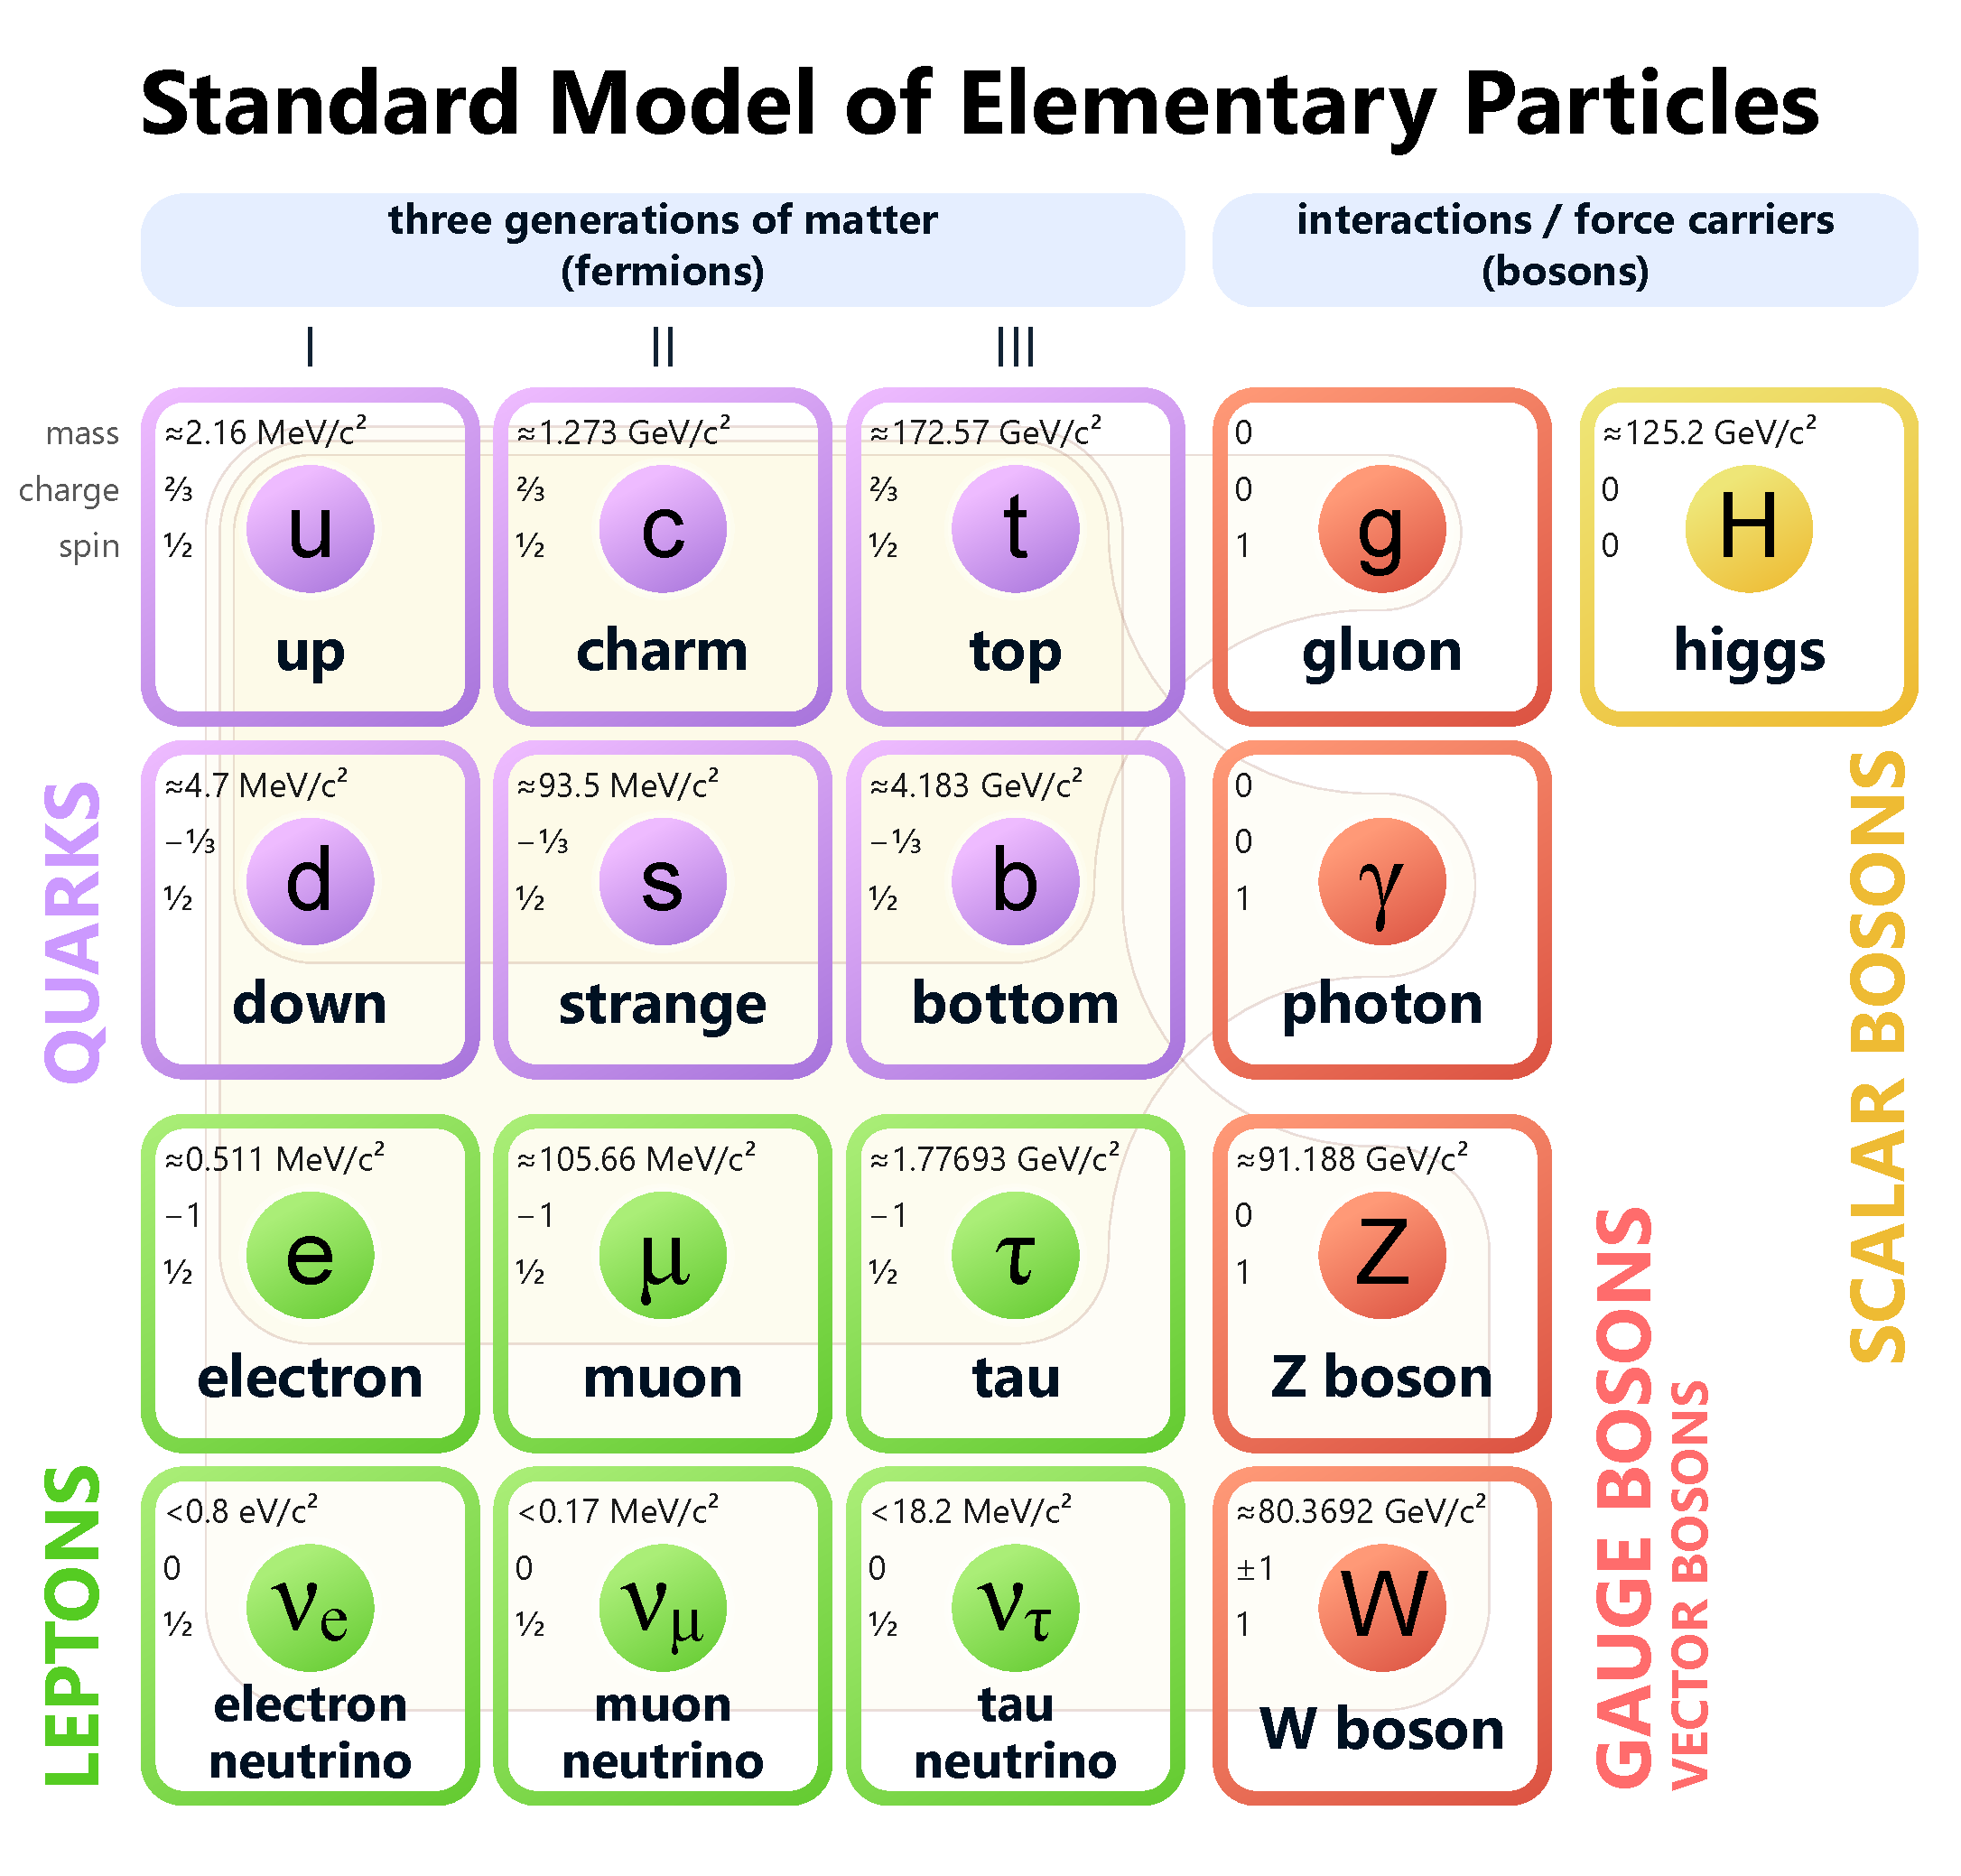
\includegraphics[width=0.8\linewidth]{res/fig/1-chapter/1-Standard_Model_of_Elementary_Particles.pdf}
        \caption{Schema delle particelle elementari presenti nel Modello Standard con relativa massa, carica e spin~\cite{Wikimedia_Standard_Model}.}
        \label{fig:1-standard-model}
    \end{figure}

    In seguito troviamo le particelle mediatrici delle interazioni fondamentali. Queste particelle hanno spin 1 e sono dette \textit{bosoni}, vettore o di gauge, poiché seguono la statistica di Bose-Einstein e corrispondono alle tre interazioni fondamentali spiegate dal Modello Standard: otto gluoni $g$ mediatori dell'interazione forte, ciascuno con tre cariche di colore possibili, il fotone $\gamma$ mediatore dell'interazione elettromagnetica e i bosoni $Z^0$ e $W^\pm$ mediatori dell'interazione debole.

    Infine nel 2012 al CERN di Ginevra è stato scoperto dagli esperimenti ATLAS \cite{ATLAS_2012} e CMS \cite{CMS_2012} un bosone scalare di spin 0 chiamato bosone di Higgs $H$ associato al campo di Higgs col quale interagiscono tutte le particelle massive, fermioniche o bosoniche, per ottenere la loro massa tramite un meccanismo detto di \textit{rottura spontanea della simmetria} ipotizzato nel 1964 da F. Englert e R. Brout \cite{Englert_1964}, Peter W. Higgs \cite{Higgs_1964} e G. S. Guralnik, C. R. Hagen e T. W. B. Kibble \cite{GHK_1964}.
    
    È bene precisare che quelle presentate non sono particelle in senso classico, ma si fa sempre riferimento a campi quantizzati in cui i campi materiali possiedono cariche interne che permettono l'accoppiamento coi relativi campi di forza. Le teorie che compongono il Modello Standard sono teorie di campo quantizzato (Quantum Field Theory QFT): la \textit{Teoria Elettrodebole} che generalizza la Elettrodinamica Quantistica (Quantum Electrodynamics QED) e spiega i fenomeni elettromagnetici e di interazione debole e la \textit{Cromodinamica Quantistica} (Quantum Chromodynamics QCD) che spiega l'interazione tra quark attraverso lo scambio di gluoni. Ancora però non siamo capaci di descrivere in senso quantistico l'ultima interazione naturale, quella gravitazionale, per questo non presente nel modello.

    La fisica delle particelle studia fenomeni che coinvolgono corpi di dimensioni infinitesime a velocità prossime a quella della luce, è naturale quindi che il formalismo matematico del Modello Standard sia quello delle teorie di campo quantizzato che rappresentano l'evoluzione della meccanica quantistica in ambito relativistico e permettono lo studio di fenomeni sia quantistici sia relativistici e la creazione e distruzione di particelle.
    
    Il concetto di campo quantizzato è associato sia alle particelle sia alle loro interazioni: le prime sono interpretate come manifestazione del relativo campo, le ultime come scambio di quanti virtuali col campo di forza relativo all'interazione in gioco. Il Modello Standard è una teoria quantistica di campo di gauge locale che nel linguaggio della teoria dei gruppi di simmetrie si indica come $SU(3)_C \times SU(2)_L \times U(1)_Y$ in cui, da sinistra, sono racchiuse le tre interazioni naturali: forte, debole e elettromagnetica.

    Le interazioni nucleari forti sono a corto raggio per cui confinate all'interno degli adroni e descritte dalla simmetria inviolata $SU(3)_C$, dove $C$ sta per colore, sulla quale poggia la \textit{Cromodinamica Quantistica} (QCD, vedi la sezione~\ref{sec:QCD}). Lo spazio di $SU(3)_C$ ha $3^2 - 1 = 8$ generatori, cioè otto bosoni di gauge di spin 1 chiamati \textit{gluoni} $g$ mediatori dell'interazione forte. Come detto prima, tra i fermioni solo i quark sono soggetti all'interazione forte ovvero possiedono la carica, di colore, di $SU(3)_C$ che può assumere tre valori convenzionalmente indicati come $red\ (r)$, $green\ (g)$ e $blue\ (b)$ e rispettivi anticolori. I quark interagiscono tra loro scambiando gluoni dotati di una doppia carica di colore: colore-anticolore, a differenza dei fotoni che sono elettricamente neutri e cioè non possiedono la carica del campo che mediano. Per questo motivo i gluoni possono interagire tra loro, mentre i fotoni no. Matematicamente questa differenza è descritta dalla non abelianità del gruppo della QCD e dalla abelianità di quello della QED.

    Le interazioni debole e elettromagnetica sono descritte e unificate dalla simmetria $SU(2)_L \times U(1)_Y$, dove $L$ sta per leptoni e $Y$ per hypercharge, ipercarica, e dal meccanismo di Higgs di rottura della simmetria che permette alle particelle di acquisire la loro massa. Nella forma più semplice questo meccanismo produce 4 bosoni di gauge, vettori, di spin 1: due neutri di cui uno massivo ($Z^0$) e uno privo di massa ($\gamma$) e due carichi e massivi ($W^\pm$) più un bosone scalare di spin 0, il bosone di Higgs ($H$)~\cite{Vitale_1995}.

    \newpage

\section{Adroni e Modello a Quark (QPM)}
\label{sec:QPM}
    I dati relativi agli esperimenti di diffusione profondamente inelastica e-p suggerirono un modello fenomenologico dell'interno dell'adrone che prese il nome di \textit{modello a partoni}. Proposto da Richard Feynman nel 1969, questo modello ipotizza che i nucleoni, costituenti del nucleo atomico, non siano particelle elementari, ma siano costituiti da centri diffusori puntiformi detti partoni. In seguito i partoni vennero identificati con quark e gluoni e oggigiorno il termine \textit{partone} indica quark e gluoni costituenti di un adrone indifferentemente.
    
    Col termine \textit{adrone} indichiamo le particelle composte di quark, solitamente più pesanti dei leptoni, il cui nome deriva dal greco \textit{hadrón}, pesante, che possiedono carica di colore e che possono quindi interagire tramite forza forte. Solitamente i quark che costituiscono l'adrone vengono chiamati \textit{quark di valenza}, mentre gluoni, quark e antiquark virtuali generati dalle forze forti che uniscono i quark di valenza vengono chiamati \textit{mare}.

    Il Modello a Quark noto anche come Modello a Partoni o Modello Quark-Partone (Quark-Parton Model QPM), è un modello che descrive gli adroni come composti di quark fornendone una semplice classificazione. Poiché i quark liberi, ovvero non legati assieme all'interno di un adrone, non sono mai stati osservati, è stato \textit{postulato} che i quark siano confinati all'interno degli adroni, come verrà chiarito meglio nella sezione~\ref{sec:QCD}.

\section{La Cromodinamica Quantistica (QCD)}
\label{sec:QCD}
    Chiarita la struttura interna degli adroni, la QCD ci fornirà ora un quadro teorico più completo per descrivere le interazioni tra quark e gluoni.

    Come già accennato nella sezione~\ref{sec:SM}, la \textit{Cromodinamica Quantistica} (QCD) è la teoria di campo quantizzato che descrive l'interazione forte attraverso scambi di gluoni. È una teoria di gauge non abeliana con gruppo di simmetria $SU(3)_C$, possiede quindi 8 generatori o bosoni di gauge vettori di spin 1 mediatori dell'interazione forte, chiamati \textit{gluoni} $g$ che possiedono a loro volta una doppia carica di colore: colore-anticolore. La QCD mostra come le uniche combinazioni di quark possibili per formare un adrone siano \textit{mesoni} (coppie quark-antiquark) e \textit{barioni} (tripletti di quark e antiquark). Nonostante questo sono stati sperimentalmente osservati stati esotici di quattro e cinque quark e stati legati di soli gluoni.

    Sperimentalmente non sono mai stati osservati quark liberi a causa del cosiddetto \textit{confinamento di colore}: i quark si legano in doppietti o tripletti che devono necessariamente essere di colore bianco ovvero neutri cioè con carica di colore nulla. Il confinamento di colore prevede infatti che sia energeticamente favorevole la produzione di una ulteriore coppia quark-antiquark, chiamata \textit{jet adronico}, nel caso si tentasse la separazione tra quark e antiquark in un mesone fornendo energia, rendendo impossibile l'ottenimento di un quark libero come mostrato in figura~\ref{fig:2-hadron-jet}.

    \begin{figure}[t]
        \centering
        \includesvg[width=0.75\linewidth]{1-chapter/2-Quark_confinement}
        \caption{Rappresentazione grafica della rottura di stringa QCD nel vuoto~\cite{Wikimedia_Quark_Confinement}. La figura mostra come venga generata una coppia quark-antiquark quando un mesone riceve energia sufficiente: il gluone che lega i due quark si ``allunga'' finché non si spezza e forma una nuova coppia quark-antiquark.}
        \label{fig:2-hadron-jet}
    \end{figure}

    Un'altra importante proprietà della QCD è la \textit{libertà asintotica} secondo la quale l'intensità dell'interazione forte è estremamente bassa ad alte scale di energia o piccole distanze; questo comporta che a brevissima distanza i quark siano sostanzialmente liberi. In regime di alte energie o piccole distanze invece l'interazione è molto meno intensa permettendo l'utilizzo di approcci di calcolo \textit{perturbativi}~\cite{BGS_2012}.

    \subsection{Cromodinamica Quantistica Perturbativa (pQCD)}
        Due sono gli approcci tradizionali alla QCD perturbativa. Il primo è il metodo detto dell'\textit{Elemento di Matrice} (Matrix Element ME)~\cite{Vitale_1995} in cui i diagrammi di Feynman sono calcolati compiutamente per ogni ordine. In linea di principio questo metodo è il più rigoroso, ma incontra grandi difficoltà già al terzo ordine, tanto che i soli calcoli ad ora disponibili si arrestano al secondo ordine perturbativo.

        Il secondo approccio è quello della Cascata di Partoni (\textit{Parton Shower} PS)~\cite{Bambah_1989}. Si tratta in questo caso di produrre un numero arbitrario di partoni che combinati tra loro generano gli eventi a più jet. Questo è possibile poiché non vengono utilizzate le espressioni complete degli elementi di matrice, ma solo delle loro approssimazioni.

        Per determinare il regime in cui la teoria perturbativa è applicabile è necessario valutare il valore di $Q^2 = - q^2$ con $q$ \textit{quadrimomento} trasferito nella collisione e segno negativo derivante dalla metrica di Minkowski~\cite{Altarelli_2004}. Nel nostro caso, per grandi valori di $Q^2$, l'interazione forte diventa meno intensa e può quindi essere trattata con metodi perturbativi rendendo così la \textit{QCD perturbativa} (perturbative QCD, pQCD) un approccio valido.

\newpage

\section{Plasma di Quark e Gluoni (QGP)}
\label{sec:QGP}
    Un modello euristico che permette di descrivere i quark confinati negli adroni è il \textit{MIT bag model} \cite{Wong_1994}. Secondo questo modello i quark sono particelle di massa nulla all'interno di una scatola di dimensioni finite e infinitamente massivi all'esterno. In questo modo il confinamento non è altro che il risultato del bilancio tra pressione esterna e interna, quest'ultima data dall'energia cinetica dei quark stessi. I gluoni scambiati tra quark sono anch'essi confinati nella scatola la cui carica di colore totale deve essere nulla.
    
    Questo modello fornisce ragioni sufficienti del perché ci aspettiamo di trovare nuove fasi della materia formata da quark oltre alla materia adronica: se la pressione esercitata dai quark interni crescesse oltre il valore della pressione esterna si verrebbe a creare un nuovo stato della materia a temperature e pressioni altissime in cui quark e gluoni non sono più legati, chiamato \textit{Plasma di Quark e Gluoni} (Quark Gluon Plasma QGP). Una rappresentazione indicativa del diagramma di fase della materia fortemente interagente è riportato in figura~\ref{fig:3-phase-diag-qgp}.
    
    \begin{figure}[h]
        \centering
        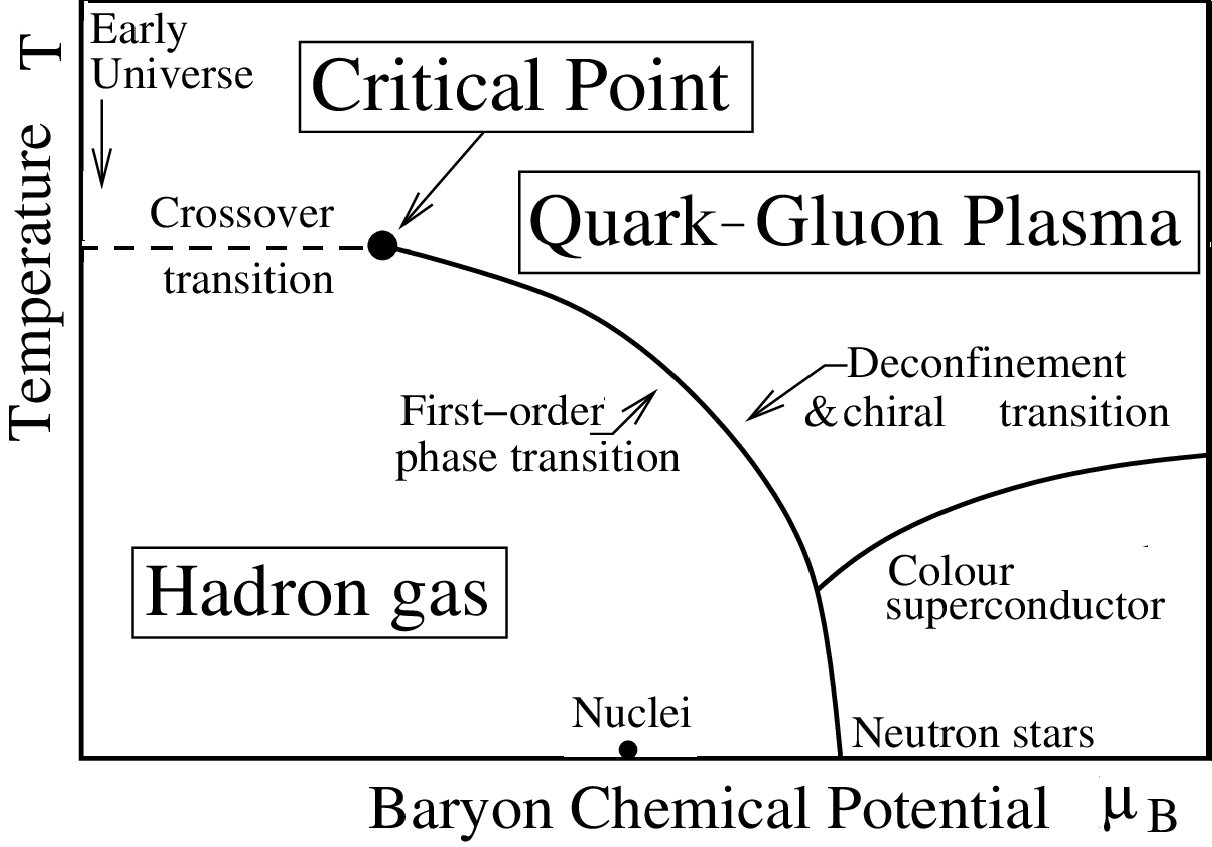
\includegraphics[width=0.7\linewidth]{res/fig/1-chapter/3-PhasDiagQGP.png}
        \caption{Diagramma di fase qualitativo della materia fortemente interagente \cite{Wikipedia_PhasDiagQGP}.}
        \label{fig:3-phase-diag-qgp}
    \end{figure}
    
    Quando il sistema raggiunge la temperatura critica $T_C \approx$ \qtyrange[range-phrase = --, range-units = single]{150}{200}{\mega \eV} avviene una transizione di fase del primo ordine tra materia adronica e QGP. La densità di energia nell'intorno di questa transizione presenta una discontinuità detta \textit{calore latente di deconfinamento}. La regione di basse temperature e alte densità è detta regione di \textit{diquark matter} o regione di \textit{superconduttività di calore}. In queste condizioni avviene la formazione di coppie di quark non neutre di colore analoghe alle coppie di Cooper dei superconduttori.

    La capacità dei barioni di ricombinare i quark per formare nuovi adroni è chiamata potenziale chimico barionico o \textit{potenziale bariochimico}, influenza la composizione di barioni e mesoni prodotti nelle collisioni ed è formulato come segue:
    
    \begin{equation}
        \mu_B = \dv{E}{N_B}.
    \end{equation}

    Un caso particolare è il QGP fortemente legato (\textit{strongly-coupled QGP} sQGP) nel quale le interazioni tra quark e gluoni sono estremamente forti e non possono essere trattate con gli approcci convenzionali basati sulla teoria perturbativa.

\section{Collisioni tra particelle}
\label{sec:COLLISION}
    Nello studio della QCD le predizioni teoriche si basano sul calcolo perturbativo di sistemi di quark e gluoni dotati di colore, carica che rappresenta i gradi di libertà a piccola distanza; le osservazioni sperimentali invece sono fatte su stati finali di adroni, ovvero stati legati di partoni in singoletto di colore. È quindi necessario analizzare i processi che portano allo stato finale cercando di descriverli con le caratteristiche dell'interazione partonica iniziale.

    Le collisioni tra ioni pesanti (A-A), ovvero tra i nuclei dei due atomi, accelerati ad energie relativistiche sono lo strumento migliore per studiare la materia nucleare in condizioni estreme di temperatura e densità di energia. È così possibile produrre numerose collisioni simultanee tra i vari nucleoni presenti nei due nuclei collidenti, creando un sistema ad altissima densità di partoni interagenti tra loro e riproducendo così in laboratorio le condizioni dell'universo primordiale frazioni di secondo dopo il Big-Bang, quando si presume che la materia in espasione si presentasse sotto forma di QGP.

    L'avvenuta formazione di uno stato di QGP può essere verificata attraverso la misura di diversi effetti come gli spettri di impulso delle particelle prodotte, la soppressione o l'aumento di produzione di stati legati di quark pesanti e la presenza di moti collettivi. È poi necessario confrontare le misure ottenute con quelle di collisioni protone-protone ($pp$) alle stesse energie per assicurarsi che lo stato prodotto in collisioni A-A non sia una semplice sovrapposizione di urti $pp$ e che si tratti effettivamente di QGP e non di un gas di adroni eccezionalmente denso.

    A complicare ulteriormente questo quadro, le differenze tra i risultati ottenuti in collisioni A-A e $pp$ potrebbero essere dovute all'utilizzo di proiettili estesi, i nuclei, nel primo caso, in particolare per le modifiche alle funzioni di distribuzione partonica nei nucleoni appartenenti ad un nucleo e alla presenza di scattering multipli prima di un hard scattering. È quindi necessario accertarsi che i risultati ottenuti in collisioni A-A non dipendano da questi effetti denominati di \textit{effetti di stato iniziale}. Per fare ciò vengono utilizzate collisioni protone-ione $p$-A.

    Negli anni sono state ottenute numerose evidenze sperimentali a favore della formazione del QGP in collisioni A-A da esperimenti ai collider SPS~\cite{NA60_2021}, RHIC e LHC~\cite{ALICE_2024}. Recentemente però in collisioni $pp$ e $p$-A sono stati \textit{osservati} gli stessi effetti normalmente associati al deconfinamento di quark, ovvero al QGP, e per questo motivo assolutamente non attesi: aumento di produzione di particelle strange, evidenze di collettività a basso impulso trasverso e presenza di correlazioni a lungo raggio con conseguenti misure di flusso ellittico e armoniche superiori. L'esperimento ALICE in particolare ha osservato un aumento della stranezza, ovvero della produzione di particelle contenenti al loro interno uno o più quark strange $s$, in funzione della molteplicità dell'evento \cite{ALICE_2008} confrontando collisioni $pp$, $p$-A e A-A in cui eventi $pp$ ad alta molteplicità mostrano risultati molto simili a quelli ottenuti in collisioni A-A \cite{RHIC_2020} \cite{ALICE_2017_pp} \cite{ALICE_2024_pp_pPb_PbPb}. Una possibile spiegazione di questo fenomeno consiste nell'assumere che anche in collisioni $pp$ ad alta molteplicità, in cui cioè avvenga più di una collisione partone-partone tra i costituenti dei due protoni interagenti, si possa creare uno stato di QGP. Questa ipotesi può spiegare la presenza di effetti collettivi negli stati finali. D'altro canto, le ridotte dimensioni del QGP eventualmente creato in collisioni $pp$ e $p$-A sarebbero in accordo con la \textit{mancata osservazione} di fenomeni di perdita di energia per partoni ad alto impulso trasverso nell'attraversare un mezzo con elevata densità di partoni liberi.

    \subsection{Collisioni tra ioni pesanti}
        L'unico metodo conosciuto per creare condizioni di temperatura e densità energetica così elevate da produrre artificialmente il QGP in laboratorio sono le collisioni tra ioni pesanti ultrarelativistici, $\beta = v/c \approx 1$.

        Le dimensioni dei nuclei degli ioni collidenti sono molto maggiori rispetto a tutte le scale proprie della fisica delle particelle elementari che appunto studia i quark costituenti dei nucleoni che a loro volta costituiscono il nucleo. Per questa ragione la \textit{geometria delle collisioni} gioca un ruolo fondamentale nell'analisi e interpretazione dei risultati sperimentali.

        Nel sistema del centro di massa, grazie alla contrazione di Lorentz nella direzione longitudinale di propagazione del fascio, i due nuclei possono essere visti nel piano trasverso come dischi sottili di raggio $2 R_A \approx 2 A^{\frac{1}{3}}$ con $A$ numero di nucleoni. Una rappresentazione grafica del processo è rappresentata in figura~\ref{fig:4-centrality}; alcune delle quantità rilevanti sono~\cite{Salgado_2009}:
        \begin{description}
            \item[\textit{parametro di impatto} $b$] distanza tra gli assi centrali dei nuclei in procinto di collidere, che caratterizza la centralità della collisione: l'urto si dirà centrale se $b$ è molto piccolo e lo scontro è pressoché frontale, si dirà invece periferico se $b$ è grande rispetto alle dimensioni delle particelle. La centralità dell'evento si esprime tipicamente in percentuali di sezione d'urto totale.
            
            \item[numero di nucleoni coinvolti] i \textit{participants}, $N_{part}$ all'interno dei nuclei collidenti ossia il numero di neutroni e protoni dei due ioni che prendono parte alla collisione. I restanti vengono chiamati spettatori, \textit{spectators}, e proseguono nella loro traiettoria quasi imperturbati. 
            
            \item[numero totale di collisioni nucleone-nucleone incoerenti] $N_{coll}$.
        \end{description}
        Numerosi modelli teorici sono stati sviluppati per descrivere le dinamiche di collisione a partire da queste quantità.

        \begin{figure}[t]
            \centering
            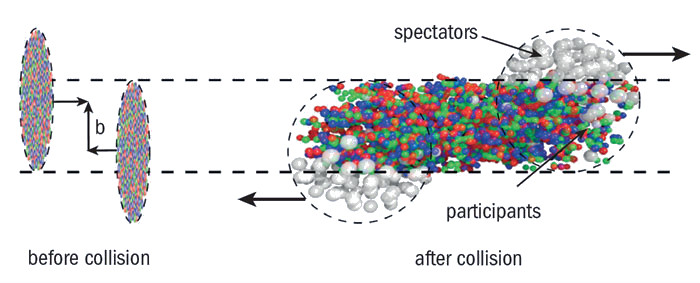
\includegraphics[width=0.8\linewidth]{res/fig/1-chapter/4-centrality.png}
            \caption{Rappresentazione geometrica della collisione tra i nuclei di due ioni pesanti~\cite{Toia_2013}. Come mostrato, la collisione può coinvolgere solamente parte dei nucleoni presenti (\textit{participants}), lasciandone fuori altri (\textit{spectators}).}
            \label{fig:4-centrality}
        \end{figure}

         In fisica subnucleare si è soliti descrivere le traiettorie delle particelle in termini della variabile \textit{rapidità} $y$ o della variabile \textit{pseudorapidità} $\eta$, definite rispettivamente come:
         \begin{equation*}
             y = \frac{1}{2} \ln(\frac{E + p_L}{E - p_L})
         \end{equation*}
        con $E = \sqrt{p^2 c^2 + m^2 c^4}$ energia relativistica e $p_L$ componente longitudinale del momento della particella rispetto all'asse del fascio e:
        \begin{equation*}
            \eta = \frac{1}{2} \ln(\frac{p + p_L}{p - p_L}) = - \ln(\tan{\frac{\theta}{2}})
        \end{equation*}
        con $\theta$ angolo tra impulso della particella e asse del fascio. Per particelle di massa nulla come il fotone rapidità e pseudorapidità coincidono, mentre per particelle massive questa corrispondenza vale solo nel limite ultrarelativistico.

\section{Evoluzione del QGP}
    Avvenuta la collisione si ha la formazione di un plasma di quark e gluoni solo nel caso in cui vengano raggiunte le condizioni critiche di temperatura e densità di energia~\cite{Andronic_2014}.
    
    Nel caso in cui le condizioni richieste non venissero raggiunte il sistema entrerebbe in \textit{evoluzione idrodinamica}, figura~\ref{fig:5-time-evol-qgp} a) a sinistra. Questo è il caso tipico delle collisioni tra protoni $pp$ o di collisioni tra ioni pesanti A-A non sufficientemente energetiche e centrali. Subito dopo la collisione vi è una breve fase \textit{pre-adronica}, in grigio, in cui i quark prodotti adronizzano in un ``vuoto'' QCD dopo la quale il sistema evolve come \textit{gas di adroni}, in sostanza attraverso processi di frammentazione. Sebbene avvenga un sostanziale incremento di pressione e temperatura non si manifesta alcun deconfinamento di partoni in questo caso.

    Nel caso in cui invece la collisione fosse sufficientemente energetica da soddisfare le condizioni di creazione del QGP, il processo rappresentato in figura~\ref{fig:5-time-evol-qgp} b) a destra è più complesso~\cite{Strazzi_2019}:
    \begin{enumerate}
        \item \textit{Pre-Equilibrium phase} ($t < \tau_0 \approx$ \qty[per-mode = symbol]{1}{\femto \meter \per \clight}): in questa fase i partoni diffondono l'uno sull'altro producendo quark e gluoni deconfinati in abbondanza. Vengono prodotte molte particelle ad elevato impulso trasverso ($p_T \gg$ \qty[per-mode = symbol]{1}{\giga \eV \per \clight}) e una grande quantità di fotoni sia reali sia virtuali che decadono in coppie leptone-antileptone.

        \item \textit{Termalizzazione} ($t \approx$ \qtyrange[range-phrase = --, range-units = single, per-mode = symbol]{1}{10}{\femto \meter \per \clight}): questa fase è caratterizzata dalle interazioni elastiche e inelastiche tra i partoni del QGP. Le interazioni inelastiche hanno la peculiarità di poter cambiare la composizione di sapore delle particelle. A causa della pressione interna il sistema all'equilibrio termico inizia ad espandersi rapidamente raffreddandosi di conseguenza e convertendosi in un gas adronico (\textit{fase mista}).

        \item \textit{Adronizzazione} ($t \approx$ \qty[per-mode = symbol]{20}{\femto \meter \per \clight}): durante l'espansione il sistema si raffredda raggiungendo il valore critico di densità che dà inizio al processo di adronizzazione in cui quark e gluoni del QGP condensano in nuovi adroni. L'interazione tra gli adroni continua finché il relativo tasso è in grado di sostenere l'espansione del QGP e raggiunto un certo valore della temperatura cessano le interazione inelastiche tra i costituenti del sistema. Dopodiché la composizione di sapore del QGP si fissa raggiungendo il congelamento chimico (\textit{chemical freeze-out}).

        \item \textit{Congelamento termico} (\textit{thermal freeze-out}): quando la densità del sistema è tale da rendere la distanza media tra gli adroni maggiore del raggio di azione dell'interazione forte, per $T_{fo} \approx$ \qty{120}{\mega \eV}, le diffusioni elastiche tra gli adroni cessano e resta fisso anche lo spettro cinematico della materia risultante.
    \end{enumerate}

    \begin{figure}[h]
        \centering
        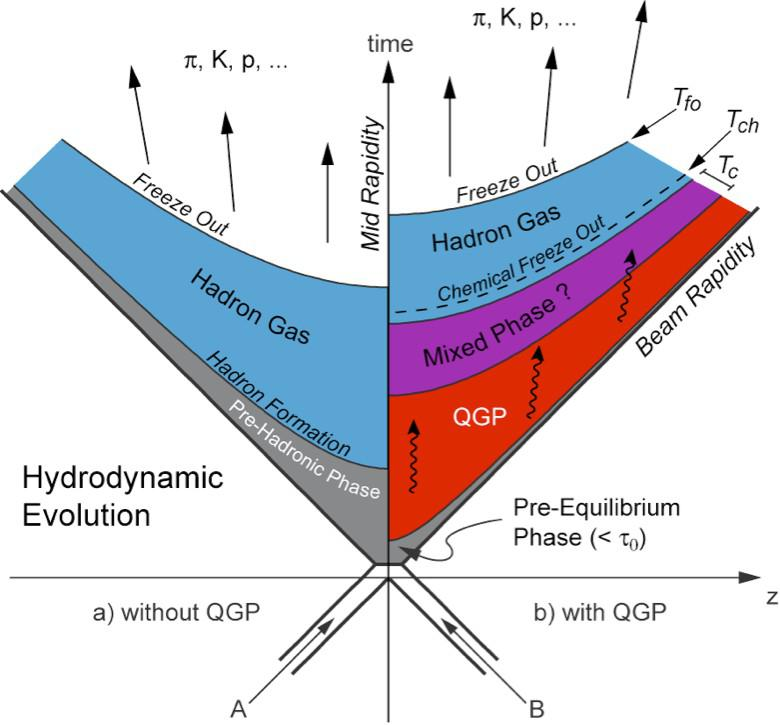
\includegraphics[width=0.65\linewidth]{res/fig/1-chapter/5-TimeEvolQGP.jpg}
        \caption{Evoluzione temporale di una collisione tra ioni pesanti in un piano simile a quello di Minkowski. a) a sinistra il caso in cui il sistema entra in evoluzione idrodinamica e diventa un gas adronico senza formazione di QGP. b) a destra il caso in cui le condizioni permettono la formazione del QGP che perdendo energia si trasforma anch'esso in gas adronico~\cite{ES_2011}.}
        \label{fig:5-time-evol-qgp}
    \end{figure}

\section{Adronizzazione di sapori pesanti in collisioni $pp$}
\label{sec:ADRONIZATIONpp}
    Nello studio delle proprietà del QGP i quark pesanti charm $c$ e bottom $b$ rivestono un ruolo fondamentale poiché in virtù della loro massa elevata vengono prodotti in collisioni \textit{hard}, ossia ad alto momento $Q^2$ trasferito, tra i partoni dei nucleoni solo nelle primissime fasi della collisione nucleo-nucleo, prima ancora che il sistema termalizzi e si formi lo stato di QGP. Questi quark quindi si propagano attraverso il sistema ultra-denso interagendo coi suoi costituenti e fornendo una \textit{misura diretta delle sue proprietà}. Per poter comprendere appieno una misura effettuata in collisioni A-A però è necessario confrontarla con la stessa misura effettuata in collisioni $pp$ e $p$-A, come chiarito nella sezione~\ref{sec:COLLISION}.

    L'adronizzazione di sapori pesanti in collisioni $pp$ attraverso il processo di \textit{frammentazione} viene descritta matematicamente attraverso il \textit{teorema di fattorizzazione}~\cite{CSS_2004}. Data la scala del momento $Q^2$ trasferito nel processo di collisione, esso consiste nel separare il contributo perturbativo ad alta energia della produzione del \textit{leading parton} dalla successiva conversione nello stato adronico a bassa energia non perturbativo. Il processo complessivo è:
    \begin{equation*}
        p + p \to h + X
    \end{equation*}
    dove l'adrone di riferimento $h$ è dato dal decadimento del partone $c$ proveniente dallo scattering $a + b$ dei partoni del protone $a + b \to c + d$.

    Possiamo ora esprimere la sezione d'urto invariante della produzione dell'adrone nel medio range di rapidità per collisioni $pp$ come:
    \begin{equation*}
        \dv{\sigma_{pp}^h}{y d^2 p_{T}} = K \sum_{abcd}{\int{\dd{x_a} \dd{x_b} f_{a}(x_a,Q^2) f_{b}(x_b,Q^2) \dv{\hat{t}} \sigma(a + b \to c + d) \frac{D_{{h}/{c}}^0}{\pi z_c}}}
    \end{equation*}
    con:
    \begin{description}
        \item[$f_i(x_i,Q^2)$] \textit{Funzioni di Distribuzione dei Partoni} (PDF) riferite ai partoni del protone.

        \item[$\dv{\hat{t}} \sigma(a + b \to c + d)$] sezione d'urto elementare perturbativa QCD della produzione della particella $c$ a partire dallo scattering dei partoni $a + b$.

        \item[$D_{{h}/{c}}^0$] \textit{Funzione di Frammentazione} (FF): elemento adimensionale che fornisce la probabilità che il partone $c$ adronizzi nell'adrone finale $h$ emettendo gluoni e trasportando una frazione del momento del partone iniziale. Le FF non sono calcolabili perturbativamente e devono essere quindi misurate sperimentalmente.
    \end{description}

    \subsection{Funzioni di Distribuzione di Partoni (PDF)}
    \label{sec:PDF}
        Le evidenze sperimentali hanno mostrato che gli adroni non sono particelle elementari puntiformi, ma sono composte da \textit{partoni}: quark e gluoni. Come detto nella sezione~\ref{sec:QPM}, i costituenti interni di un adrone possono essere divisi in \textit{quark di valenza}, ossia i quark che effettivamente determinano i numeri quantici dell'adrone come $uud$ per il protone p, e in partoni del mare o \textit{mare}, ossia tutti i restanti partoni, gluoni e quark, creati e distrutti nei processi virtuali che avvengono all'interno dell'adrone secondo la QCD.

        Consideriamo l'esempio del protone p. Denotiamo con
        \begin{description}
            \item[$q^v(x)$] la densità di probabilità di un quark di valenza,

            \item[$q^s(x)$] la densità di probabilità di un quark del mare,

            \item[$g(x)$] la densità di probabilità di un gluone,

            \item[$x$] la frazione del momento totale trasportato da un quark $q$ o un gluone $g$.
        \end{description}
        Sapendo che i quark di valenza del protone sono $uud$, otteniamo la condizione:
        \begin{equation*}
            \int_{0}^{1}{\dd{x} u^v(x)} = 2 \qquad \int_{0}^{1}{\dd{x} d^v(x)} = 1.
        \end{equation*}
        I quark del mare sono sempre prodotti in coppie $q\bar{q}$ e danno un contributo nullo al numero barionico:
        \begin{equation*}
            \int_{0}^{1}{\dd{x} [u^s(x) - \bar{u}^s(x)]} = 0 \qquad \int_{0}^{1}{\dd{x} [d^s(x) - \bar{d}^s(x)]} = 0.
        \end{equation*}
        La stessa condizione è valida per gli altri quark del mare $s^s$, $c^s$, $b^s$ e $t^s$.
        Il momento totale portato da tutti i partoni deve contribuire al momento totale, perciò si ha la condizione:
        \begin{equation*}
            \int_{0}^{1}{\dd{x} x [u^{v}(x) + d^{v}(x) + \sum_{q} (q^{s}(x) + \bar{q}^{s}(x))]} = 1
        \end{equation*}
        I quark pesanti sono inclusi nella presente trattazione, ma sono attivi solamente se la scala di energia $Q$ del sistema è superiore alla massa $m_q$ del quark pesante stesso.

        In figura \ref{fig:6-pdf-momentum-proton} sono mostrate le funzioni di distribuzione del momento dei partoni del protone a $Q^2 =$ \qty{10}{\giga \eV^2}. È interessante notare come il termine dei gluoni rappresenti circa metà del momento totale.

        \begin{figure}[h]
            \centering
            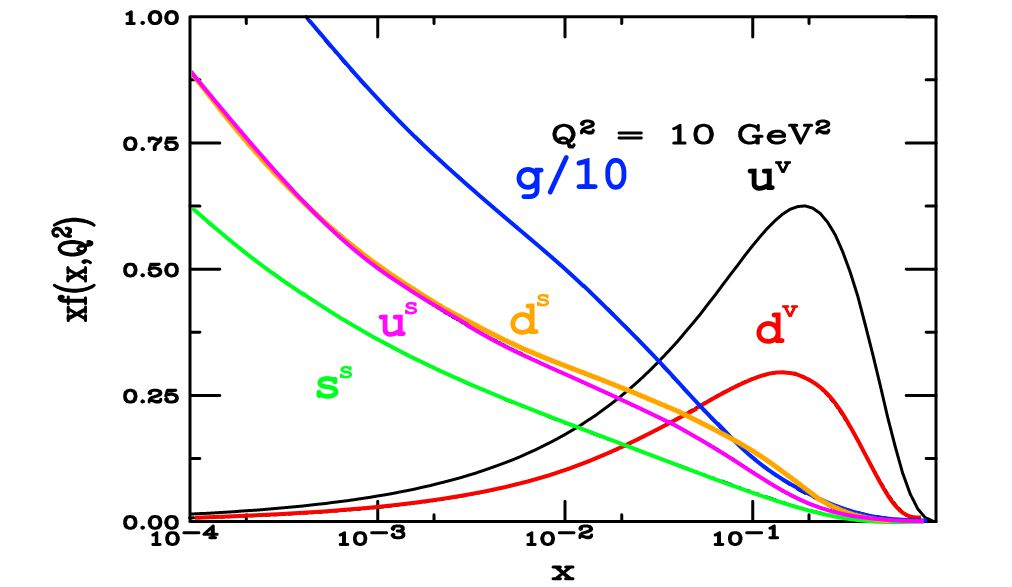
\includegraphics[width=0.71\linewidth]{res/fig/1-chapter/6-pdf-momentum-proton.jpg}
            \caption{Funzioni di distribuzione del momento dei partoni del protone $xf(x)$, secondo la parametrizzazione CTEQ6M dei partoni a $Q^2 =$ \qty{10}{\giga \eV^2}. La distribuzione dei gluoni è divisa per 10 per migliorarne la visualizzazione~\cite{Fusconi_2022}.}
            \label{fig:6-pdf-momentum-proton}
        \end{figure}

    \subsection{Funzioni di Frammentazione (FF)}
        Per comprendere meglio le Funzioni di Frammentazione consideriamo il processo di annichilazione di un sistema elettrone-positrone per produrre una coppia quark-antiquark~\cite{Vogt_2007}
        \begin{equation*}
            e^{-} e^{+} \to q \bar{q}.
        \end{equation*}
        Se l'energia della collisione è $Q$ allora l'energia del fascio è $E_f = Q/2$, in maniera simmetrica, e i quark prodotti hanno energia $E_q = E_f$. Dunque se l'adrone $h$ dello stato finale ha energia $E_h$, questo porterà una frazione di energia data da
        \begin{equation*}
            z = \frac{E_h}{E_q} = \frac{2 E_h}{Q}.
        \end{equation*}
        La sezione d'urto differenziale per la produzione di adroni come funzione di $z$ è:
        \begin{equation*}
            \dv{\sigma(e^{-} e^{+} \to h X)}{z} = \sum_{q}{\sigma(e^{-}e^{+} \to q \bar{q})[D_{q}^{h}(z) + D_{\bar{q}}^{h}(z)]}.
        \end{equation*}
        Questa formula è data dall'applicazione del teorema di fattorizzazione senza le PDF e giustificata dal fatto che gli elettroni sono particelle elementari. La Funzione di Frammentazione $D_{q}^{h}(z)$ rappresenta la probabilità che l'adrone $h$ dello stato finale trasporti una frazione $z$ del momento iniziale del quark, descrive quindi la transizione partone-adrone nello stesso modo in cui la PDF descrive la struttura partonica di un adrone. Per quanto detto la somma delle energie di tutti gli adroni prodotti deve formare l'energia del quark iniziale:
        \begin{equation*}
            \sum_{h}{\int_{0}^{1}{\dd{z} z D_{q}^{h}(z)}} = \sum_{h}{ \int_{0}^{1}{\dd{z} z D_{\bar{q}}^{h}(z)}} = 1.
        \end{equation*}
        La molteplicità di $h$ è data dalla somma delle probabilità di produrre $h$ da tutti i possibili quark e antiquark:
        \begin{equation*}
            n_{h} = \sum_{q}{\int_{z_{\min}}^{1} \dd{z} [D_{q}^{h}(z) + D_{\bar{q}}^{h}(z)]}
        \end{equation*}
        dove $z_{\min} = 2 m_{h} / Q$ è l'energia di soglia necessaria per produrre un adrone di massa $m_{h}$.

        Le FF possono avere diverse parametrizzazioni. Spesso è utilizzata quella in cui
        \begin{equation*}
            D_{q}^{h}(z) = N \frac{(1-z)^n}{z}
        \end{equation*}
        con $N$ e $n$ costanti specifiche per un dato adrone $h$. I parametri sono ottenuti sperimentalmente dal fit dell'immensa molte di dati disponibile per collisioni $e^{-} e^{+}$.

        Si ipotizza che le Funzioni di Frammentazione siano universali, pertanto una volta calcolati i parametri per le collisioni $e^{-} e^{+}$, questi dovrebbero essere applicabili in altri casi come le collisioni $ep$, $pp$ e $p\bar{p}$.

\section{Adronizzazione di sapori pesanti in collisioni A-A}
    Fin dalle prime osservazioni di produzione di adroni in collisioni tra ioni pesanti fu evidente che il processo di \textit{adronizzazione} fosse diverso dalla pura \textit{frammentazione} nel vuoto. I modelli che tentano di spiegare questa differenza considerano che avvenga in concomitanza anche un secondo meccanismo chiamato \textit{ricombinazione} o \textit{coalescenza}. La differenza tra i due processi è che nella
    \begin{description}
        \item[frammentazione] il momento iniziale è distribuito tra i frammenti, mentre nella

        \item[ricombinazione] due o tre partoni vicini nello spazio delle fasi (posizione e momento) producono un adrone con momento trasverso pari alla somma dei momenti dei partoni iniziali
    \end{description}
    come mostrato il figura \ref{fig:7-fragm-recom}.

    Il calcolo degli effetti di ricombinazione nelle collisioni tra ioni pesanti è particolarmente complesso poiché non è possibile scrivere la funzione d'onda di tutti i partoni che costituiscono il QGP.

    La probabilità di trovare due o tre partoni vicini nello spazio delle fasi diminuisce all'aumentare del momento trasverso dell'adrone nello stato finale, per questo la ricombinazione contribuisce meno ad \textit{alti impulsi trasversi} $p_T$ dove la frammentazione risulta il fenomeno dominante. Inoltre l'effetto della ricombinazione è più significativo \textit{in collisioni centrali} poiché queste ultime favoriscono maggiormente la transizione a QGP, mentre la frammentazione è tipica delle \textit{collisioni periferiche}.

\newpage

    \begin{figure}[h]
        \centering
        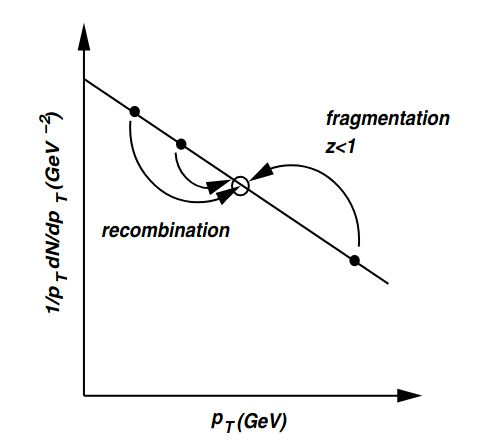
\includegraphics[width=0.6\linewidth]{res/fig/1-chapter/7-fragm-recom.jpg}
        \caption{I meccanismi di ricombinazione e frammentazione in atto per creare lo stesso adrone nello stato finale in funzione dell'impulso trasverso $p_{T}$~\cite{Vogt_2007}.}
        \label{fig:7-fragm-recom}
    \end{figure}

\newpage

\section{Rapporto di produzione barione/mesone}
\label{sec:BARIONE/MESONE}
    Come detto nella sezione~\ref{sec:ADRONIZATIONpp}, i quark pesanti sono di grande interesse per lo studio delle proprietà del QGP poiché, creati in coppia solo nei primissimi istanti della collisione, attraversano il sistema durante tutte le fasi della sua evoluzione interagendo coi suoi costituenti e fornendo una misura diretta delle sue proprietà.

    Alcuni modelli teorici prevedono una \textit{produzione di barioni}, stati legati di 3 quark, \textit{più abbondante} di quella di mesoni, stati legati di 2 quark, in un mezzo denso deconfinato (QGP) per effetto di processi di adronizzazione per \textit{ricombinazione} (coalescenza) tra quark che si aggiungono al processo di adronizzazione per \textit{frammentazione}. Lo studio del \textit{rapporto di produzione barioni/mesoni} in collisioni A-A e pp è quindi un importante strumento per studiare l'effetto del QGP sull'adronizzazione dei quark.

    $\Lambda_{c}^{+}(udc)$ e $D^{0}(c \bar{u})$ sono rispettivamente il barione e il mesone più leggeri contenenti un quark charm e possono essere identificati in un ampio intervallo di momento, per questo si prestano molto bene per valutare il rapporto di produzione barione/mesone nelle diverse collisioni.

    \subsection{Adroni charmati in collisioni \ch{Pb}-\ch{Pb} a $\sqrt{s_{NN}} =$ \qty{5.02}{\tera \eV}}
        Contrariamente a quanto atteso, i valori misurati del rapporto barione/mesone mostrati in figura~\ref{fig:8-ALICE-pp13TeV-pp5.02TeV-pPb5.02TeV-PbPb5.02TeV} \textit{non} differiscono in maniera significativa tra di loro e in particolare \textit{non} si osserva il consistente aumento della produzione di barioni charmati, riferito alla produzione di mesoni charmati, previsto dall'insorgere di meccanismi di \textit{ricombinazione} in collisioni A-A (qui \ch{Pb}-\ch{Pb}). Infatti, nei processi di \textit{ricombinazione} o coalescenza, la formazione di un barione è molto \textit{meno} sfavorita rispetto alla formazione di un mesone a differenza dei processi di \textit{frammentazione} che invece la disincentivano. Questo porterebbe a \textit{prevedere} un valore del rapporto barione/mesone \textit{maggiore} in collisioni A-A~\cite{Strazzi_2019} come accennato sopra, sezione~\ref{sec:BARIONE/MESONE}. Una possibile spiegazione è che tali o simili meccanismi siano \textit{già} presenti e importanti, soprattutto a basso $p_T$, \textit{anche} in collisioni pp e $p$-A alle energie di LHC. L'andamento del rapporto in funzione della molteplicità dimostra che, se presenti, tali meccanismi sono \textit{già} all’opera anche a basse molteplicità.

        Con l'espressione \textit{molteplicità} o \textit{classi di molteplicità} intendiamo il numero di particelle secondarie prodotte in un evento. Questo termine aiuta a organizzare e analizzare i dati delle collisioni: gli eventi con alta molteplicità possono essere più complessi, ma potenzialmente più informativi rispetto a quelli a bassa molteplicità. Questa categorizzazione permette una migliore comprensione dei processi fisici coinvolti.

\newpage
        
        \begin{figure}[t]
            \centering
            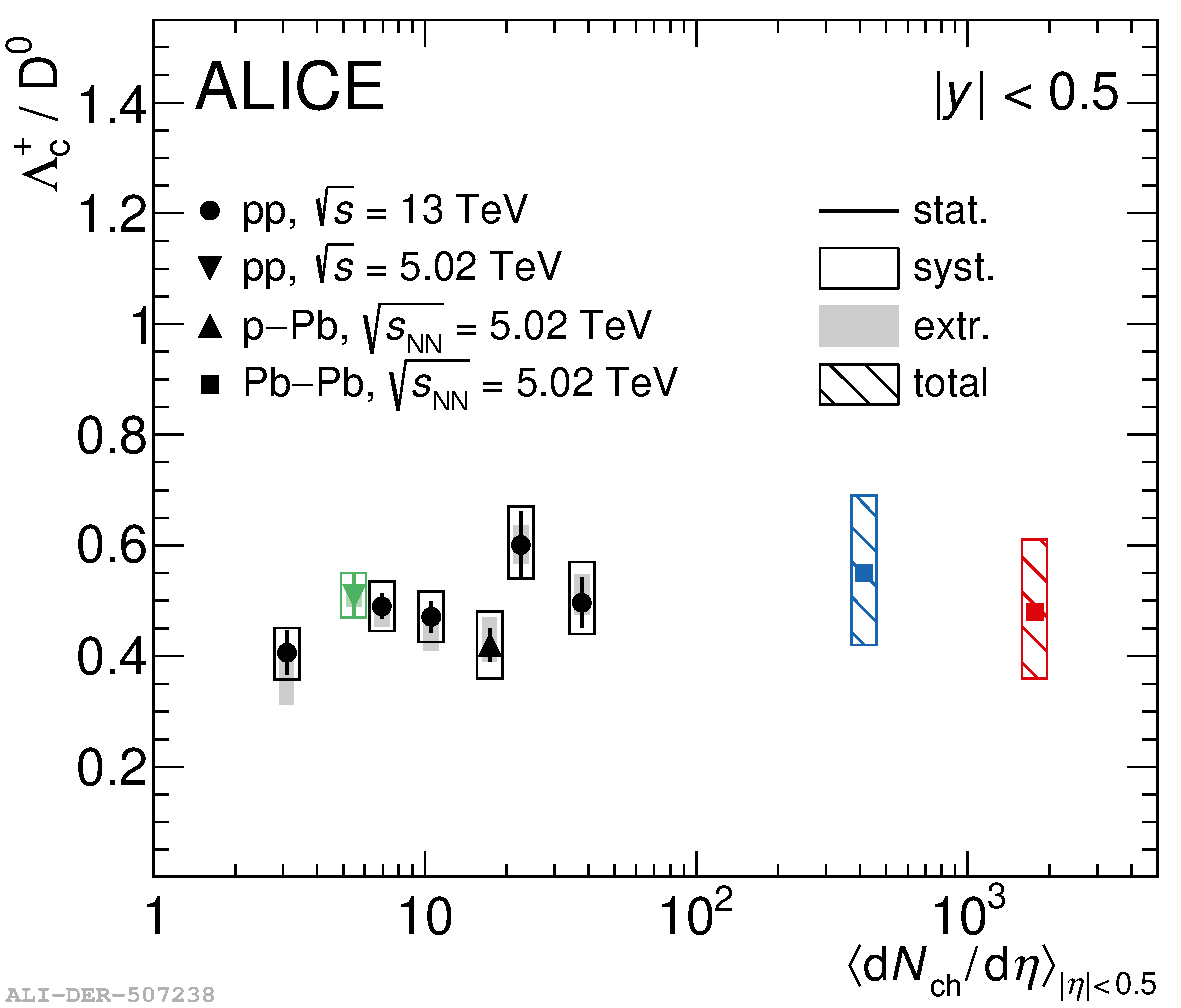
\includegraphics[width=0.65\linewidth]{res/fig/1-chapter/8-ALICE-pp13TeV-pp5.02TeV-pPb5.02TeV-PbPb5.02TeV.pdf}
            \caption{Valore del rapporto barione/mesone $\Lambda_{c}^{+}/D^{0}$ misurato dall'esperimento ALICE a LHC integrato su tutto lo spettro degli impulsi trasversi $p_{T}$ del barione $\Lambda_{c}^{+}$ (sono stati utilizzati valori estrapolati dove non erano presenti misure sperimentali) per diversi sistemi collidenti: protone-protone pp, protone-nucleo $p$-\ch{Pb} e nucleo-nucleo \ch{Pb}-\ch{Pb}, sia centrali sia periferici, in funzione della molteplicità~\cite{Kalteyer_ALICE_2022}. Si può notare come il rapporto sia praticamente compatibile per tutti i tipi di collisioni entro gli errori sperimentali.}
            \label{fig:8-ALICE-pp13TeV-pp5.02TeV-pPb5.02TeV-PbPb5.02TeV}
        \end{figure}

    \subsection%
    [Adroni charmati in collisioni pp a $\sqrt{s} =$ \qty{5.02}{\tera \eV} e a $\sqrt{s} =$ \qty{13}{\tera \eV}]%
    {Adroni charmati in collisioni pp a $\sqrt{s} =$ \qty{5.02}{\tera \eV} e a \\ $\sqrt{s} =$ \qty{13}{\tera \eV}}
        I valori del rapporto di produzione $\Lambda_{c}^{+}/D^{0}$ misurati in collisioni $pp$ alle energie di LHC risultano significativamente \textit{maggiori} rispetto a quanto misurato in collisioni ep e $e^{+} e^{-}$ e soprattutto rispetto a modelli teorici che assumono \textit{solo} processi di frammentazione e utilizzano funzioni di frammentazione (FF) basate su tali esperimenti. Questi modelli prevedono un valore del rapporto di circa \num{0.1}, con una debole dipendenza dal valore dell'impulso trasverso, significativamente inferiore al valore compreso tra \num{0.4} e \num{0.6} misurato in ALICE~\cite{ALICE_2018_pp7Tev_pPb5.02TeV}~\cite{ALICE_2021_pp5.02TeV_pPb5.02TeV_prod}~\cite{ALICE_2021_pp5.02TeV_pPb5.02TeV_prod_ratio}~\cite{ALICE_2022_pp13TeV} a bassi lavori di $p_{T}$ (figura~\ref{fig:9-ALICE-pp5.02TeV-pp7TeV-pp13TeV}). Questa discrepanza può essere interpretata come una indicazione del fatto che le probabilità che un quark charm adronizzi in uno specifico adrone charmato, ovvero le Funzioni di Frammentazione (FF), \textit{non} siano universali come ritenuto fino ad ora, ma dipendano dalle caratteristiche del sistema collidente.
        
        Il rapporto $\Lambda_{c}^{+}/D^{0}$ in funzione dell'impulso trasverso sembra inoltre variare se considerato in diverse \textit{classi di molteplicità} (figura~\ref{fig:8-ALICE-pp13TeV-pp5.02TeV-pPb5.02TeV-PbPb5.02TeV}), con il risultato, per collisioni pp ad elevata molteplicità, che si avvicina molto a quanto ottenuto in collisioni \ch{Pb}-\ch{Pb} ad energie del centro di massa nucleone-nucleone di \qty{5.02}{\tera \eV}.

        I rapporti di produzione misurati da ALICE nel range di rapidità centrali $\abs{\eta} <$ \num{0.9} in collisioni $pp$ a diverse energie del centro di massa riportati in figura~\ref{fig:9-ALICE-pp5.02TeV-pp7TeV-pp13TeV} mostrano un certo \textit{accordo} per i valori di impulso \textit{fuori} dal bin $p_{T} =$ \qtyrange[range-phrase = {,}, range-units = single, per-mode = symbol, range-units = bracket, range-open-bracket = [, range-close-bracket = ]]{0}{1}{\giga \eV \per \clight}, con un andamento descrescente, mentre i valori al suo \textit{interno}, calcolati unicamente attraverso il canale di decadimento $\Lambda_{c}^{+} \to p K_{S}^{0}$, sono molto diversi. I risultati espressi in intervalli di $p_{T}$ sono compatibili entro gli errori sperimentali. In effetti l'analisi dei decadimenti a basso impulso trasverso è particolarmente delicata.

        \begin{figure}[h]
            \centering
            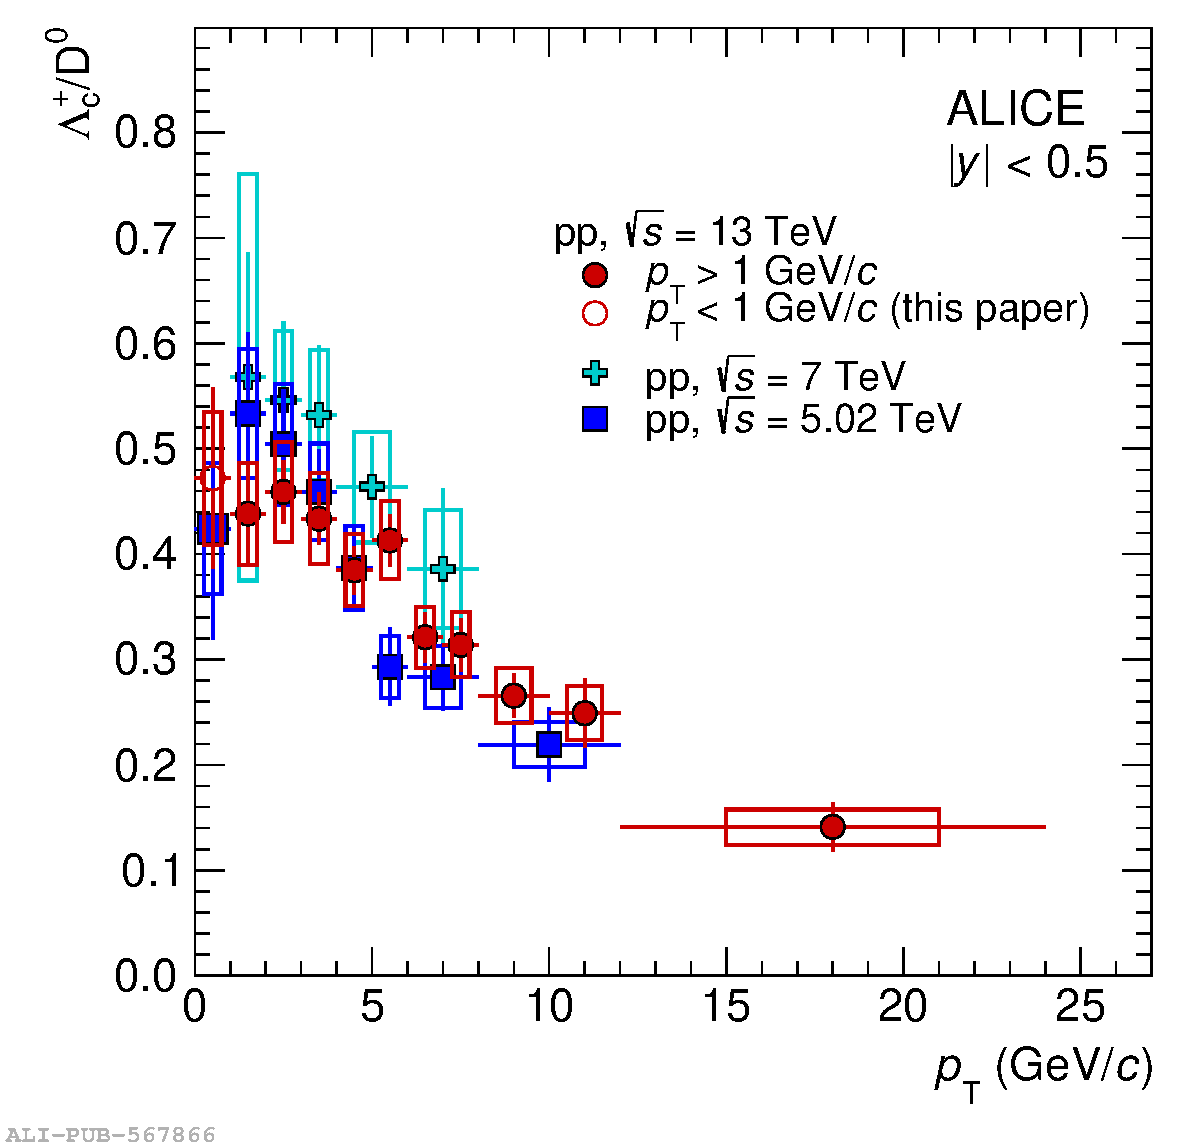
\includegraphics[width=0.65\linewidth]{res/fig/1-chapter/9-ALICE-pp5.02TeV-pp7TeV-pp13TeV.pdf}
            \caption{Rapporto di produzione degli adroni charmati $\Lambda_{c}^{+}$ e $D^{0}$ in funzione dell'impulso trasverso $p_{T}$ in collisioni pp a energia cinetica nel centro di massa di $\sqrt{s} =$ \qty{5.02}{\tera \eV}, $\sqrt{s} =$ \qty{7}{\tera \eV} e $\sqrt{s} =$ \qty{13}{\tera \eV} misurati col rivelatore ALICE a LHC \cite{ALICE_2023_pp5.02TeV_pp7TeV_pp13TeV}.}
            \label{fig:9-ALICE-pp5.02TeV-pp7TeV-pp13TeV}
        \end{figure}

        Le misure sperimentali prodotte dall'esperimento ALICE sono state confrontate con diversi modelli teorici e fenomenologici, al fine di verificarne l'attendibilità e la capacità di riprodurre i dati sperimentali. I modelli teorici riportati in figura~\ref{fig:10-ALICE-pp13TeV} sono:
        \begin{description}
            \item[PYTHIA 8.243 Monash 2013]~\cite{SCR_2014} un generatore Monte Carlo (MC) che implementa \textit{solo} processi di \textit{frammentazione} con FF per adroni charmati basate sulle misurazioni ottenute con collisioni $e^{+} e^{-}$. Predice un rapporto $\Lambda_{c}^{+}/D^{0}$ di circa \num{0.1} con una debole dipendenza da $p_{T}$ e costituisce una grossa sottostima dei dati sperimentali, soprattutto a bassi range di impulso trasverso.

            \item[PYTHIA 8.243]~\cite{CS_2015} un generatore MC che implementa la \textit{riconnessione di colore}. Questo modello di adronizzazione è basato sul \textit{modello a stringhe di Lund}. Sono presenti tre possibili modalità che introducono vincoli più o meno restrittivi sulla generazione: Mode 0 senza vincoli, Mode 2 con vincoli stretti, Mode 3 con vincoli più larghi. Questo modello predice \textit{piuttosto bene} l’andamento del rapporto $\Lambda_{c}^{+}/D^{0}$ in particolare nella Mode 0.

            \item[SHM+RQM] (Statistical Hadronization Model - Relativistic Quark Model)~\cite{MR_2019} un modello che calcola le frazioni di adroni charmati basandosi su \textit{densità termiche}, dunque dipendenti dalla massa dello stato e dal fattore di degenerazione di spin. Fa uso di ulteriori stati barionici eccitati ancora non misurati, ma che si assume esistano secondo il modello relativistico dei quark (RQM). Secondo tale modello, l'incremento nella produzione di barioni charmati non è dovuto a $\Lambda_{c}^{+}$ primarie, ma a decadimenti di stati barionici di massa più elevata ($\Lambda_{c}^{+}$ di feed-down). Le previsioni di questo modello sono buone per tutti i range di $p_{T}$.

            \item[Catania]~\cite{PMDCG_2018} un modello che assume che anche in collisioni pp si possa creare uno stato di QGP e che dunque l’adronizzazione avvenga sia per \textit{frammentazione} che per \textit{ricombinazione} (coalescenza).
            
            \item[QCM]~\cite{QCM} è un modello che ipotizza la formazione di adroni charmati, a basso $p_{T}$, dalla combinazione di quark charm con quark più leggeri ($u$, $d$, $s$) che si muovono alla stessa velocità.

            \item[POWLANG]~\cite{POWLANG} similmente al modello Catania, assume la creazione di uno stato di QGP anche in collisioni $pp$ ed utilizza lo stesso meccanismo di adronizzazione in-medium sviluppato per descrivere i risultati ottenuti con collisioni Pb-Pb. In questo modello, la formazione di barioni charmati avviene dalla combinazione di quark charm con stati di diquark leggeri eccitati presenti nel plasma. Tra i vari modelli proposti, questo è quello che riproduce in maniera meno accurata l'andamento del rapporto $\Lambda_{c}^{+}/D^{0}$ in funzione di $p_{T}$.
            
        \end{description}
        Questi modelli, escluso PYTHIA 8.243 Monash 2013, forniscono previsioni simili in quasi tutto il range di impulso trasverso $p_{T}$, tranne nel bin \qtyrange[range-phrase = {,}, range-units = single, per-mode = symbol, range-units = bracket, range-open-bracket = [, range-close-bracket = ]]{0}{1}{\giga \eV \per \clight}. L’\textit{analisi dati in questo range} è dunque molto importante, perché permette di \textit{distinguere i modelli teorici} più affidabili da quelli che lo sono meno. È tuttavia un’analisi molto difficile a causa del bassissimo rapporto segnale su fondo. Inoltre, come si può vedere in figura \ref{fig:10-ALICE-pp13TeV}, l’errore statistico e quello sistematico sono significativi, il che rende la misura sperimentale meno attendibile e di difficile interpretazione.

        \begin{figure}[h]
            \centering
            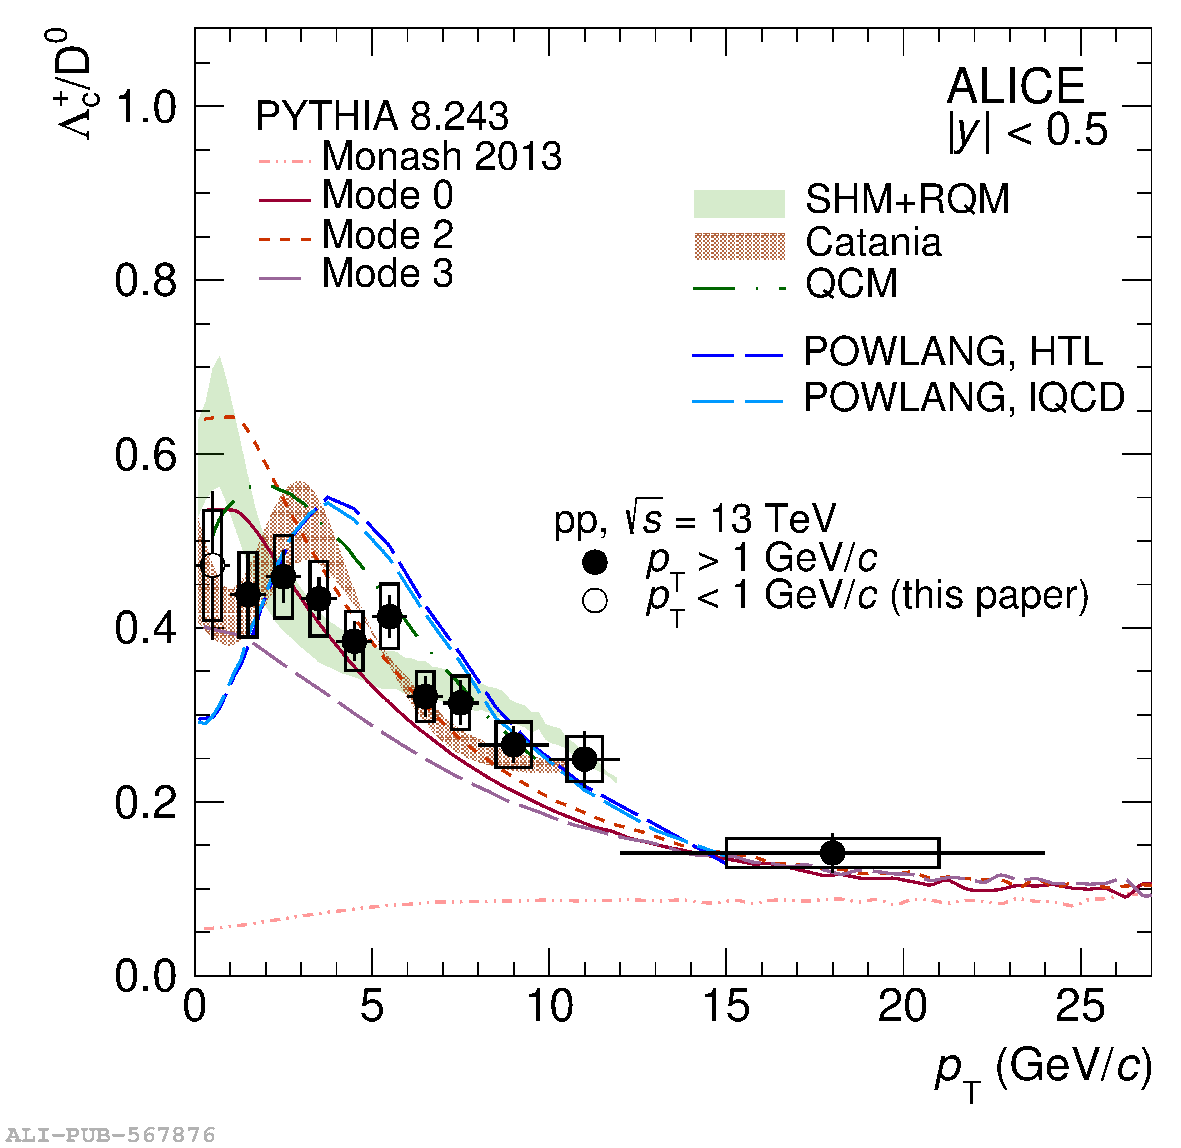
\includegraphics[width=0.65\linewidth]{res/fig/1-chapter/10-ALICE-pp13TeV.pdf}
            \caption{Rapporto di produzione $\Lambda_{c}^{+}/D^{0}$ in funzione dell'impulso trasverso $p_{T}$ in collisioni pp a $\sqrt{s} =$ \qty{13}{\tera \eV} confrontato con diversi modelli teorici \cite{ALICE_2023_pp13TeV}.}
            \label{fig:10-ALICE-pp13TeV}
        \end{figure}
        %-----------------------------CAPITOLO 2
        \chapter{Esperimento ALICE}

\section{LHC: Large Hadron Collider}

\section{ALICE: A Large Ion Collider Experiment}

    \subsection{Considerazioni sulla costruzione}

    \subsection{PID: Particle Identification}

\section{ITS: Inner Tracking System}

\section{TPC: Time Projection Chamber}

\section{TOF: Time Of Flight}
        %-----------------------------CAPITOLO 3
        \chapter{Terzo}
Terzo

\begin{figure}[h]
    \centering
    \includesvg[width=1\columnwidth]{res/fig/3-chapter/vars_histogram}
    \caption{Caption}
    \label{fig:enter-label}
\end{figure}
        %-----------------------------APPENDICE
        %\appendix


    %---------------------------------BACKMATTER
    \backmatter{}
    % pulisce la pagina
    % numero pagina immutato
    % no numerazione capitoli
        %-----------------------------BIBLIOGRAFIA
        \printbibliography[heading=bibintoc]

\begin{comment}
    % SE BIBLIOGRAFIA MANUALE
    % Per mandare nell’indice generale il titolo della bibliografia del documento per la classe book e report
    %\cleardoublepage
    % fa cominciare la bibliografia in una pagina nuova dispari e assegna alla corrispondente voce nell’indice il numero di pagina corretto
    \phantomsection
    % va dato solo se è caricato anche hyperref, serve affiché la voce Bibliografia nell'indice porti alla pagina della Bibliografia
    \addcontentsline{toc}{chapter}{\bibname}
    
    \printbibliography
\end{comment}

\begin{comment}
    BIBLIOGRAFIA
    Elenco di opere scritte o di altro tipo che di solito occupa una sezione autonoma del documento con un titolo (in genere) omonimo.
    ------------------------------------------------
    RIERIMENTO BIBLIOGRAFICO
    Serie di dati che permette di identificare ed eventualmente reperire un’opera. L’insieme dei riferimenti bibliografici costituisce la bibliografia di un documento.
    
    STILE BIBLIOGRAFICO
    Modalità generale adottata per presentare al lettore i riferimenti bibliografici.
    ------------------------------------------------
    CITAZIONE BIBLIOGRAFICA
    Indicazione sintetica, data nel corpo del documento, che rinvia il lettore a un riferimento bibliografico.
    
    SCHEMA DI CITAZIONE
    Modalità generale adottata per presentare al lettore una citazione bibliografica.
\end{comment}
        %-----------------------------RINGRAZIAMENTI
        %%---------------------------------RINGRAZIAMENTI
% PRIMA DEL CLU
Alla fine del percorso di questi 3 anni e di un nuovo percorso della magistrale che già è iniziato (e per il quale sono già indietro) desidero ringraziare le persone che mi hanno accompagnato e mi sono state donate in questo cammino e per la grandezza di quanto è accaduto nella mia vita. Perdonatemi se dimenticherò qualcuno!

Vorrei innanzitutto ringraziare la mia \textit{famiglia} che mi è sempre stata vicino, supportato, sostenuto e creduto in me. Grazie \textbf{Mamma}, \textbf{Papà}, \textbf{Lorenzo} e \textbf{Nonna Giovanna} e \textbf{Nonno Gianni} che mi guardi da lassù e grazie anche ai nonni di Bologna \textbf{Ettore} e \textbf{Valeria} e anche agli \textbf{zii}.

Grazie ai miei prof del \textit{liceo} che mi hanno \textit{armato} a sufficienza per affrontare le sfide del mondo e mostrato quanto grande può essere la passione per l'educazione (che è passione per l'uomo!): \textbf{Mara Ferroni}, \textbf{Paolo Giglioli}, \textbf{Enrica Spadanuda}, \textbf{Giovanni Battista Nicotra}, \textbf{Roberto Mastri}, \textbf{Lorenzo Raggi}, \textbf{Francesco Severi}, \textbf{Don Marco Ruffini} e tutti gli altri che ho incontrato al Liceo Malpighi di Bologna.

Grazie anche ai pochi (ma buoni) amici di \textit{GS} Bologna che mi hanno fatto incontrare e conoscere il Movimento prima a scuola poi a GS perché attraverso la loro proposta è passato Qualcosa di molto più grande, loro sono stati strumento e servi: \textbf{Batti}, \textbf{Mike}, \textbf{Alys}, \textbf{Ross}, \textbf{MK}, \textbf{Lea}, \textbf{Lodo}, \textbf{Giudi}, \textbf{Giuse}, \textbf{Fede}, \textbf{Bara}, \textbf{Mens}, \textbf{Sal} e tutti gli altri.

Ringrazio il \textbf{prof Alici} per la grande professionalità e serietà che ha messo nell'assistermi in questo lavoro anche nei momenti più critici e per la grande disponibilità umana che ha nei confronti degli studenti.

\begin{verse}
    \textit{Perché i miei pensieri non sono i vostri pensieri, \\
    le vostre vie non sono le mie vie - oracolo del Signore. \\
    Quanto il cielo sovrasta la terra, \\
    tanto le mie vie sovrastano le vostre vie, \\
    i miei pensieri sovrastano i vostri pensieri. \\
    Come infatti la pioggia e la neve \\
    scendono dal cielo e non vi ritornano \\
    senza avere irrigato la terra, \\
    senza averla fecondata e fatta germogliare, \\
    perché dia il seme al seminatore \\
    e pane da mangiare, \\
    così sarà della parola \\
    uscita dalla mia bocca: \\
    non ritornerà a me senza effetto, \\
    senza aver operato ciò che desidero \\
    e senza aver compiuto ciò per cui l'ho mandata.} \\
    Isaia 55, 8-11
\end{verse}

% ARRIVO AL CLU E VECCHI
Il mio arrivo al \textit{CLU} di Bologna non è stato facile, è stato un incontro-scontro, sicuramente non era come me lo sarei aspettato: era pieno di persone che mi volevano bene, ma in un modo da me inaspettato e grandissimo e sicuramente non secondo la mia misura per cui è stato molto difficile \textit{accogliere} questa modalità nuova.

Grazie \textbf{Don Marco} per la serietà con cui mi hai sempre guardato e per avermi invitato fin da subito a conoscere i più grandi della mia facoltà e a buttarmi e implicarmi in un'esperienza che ha solo fatto più grande la mia vita.

Grazie agli amici più \textit{grandi} che ho conosciuto e stimato fin dal primo istante.

Grazie \textbf{Gigi} per l'unità che vivi e testimoni nella tua vita, sei come un padre per me.

Grazie \textbf{Gae} per avermi accolto fin dall'inizio e avermi buttato dentro (quasi troppo) alla vita di Scienze.

Grazie \textbf{Flex} perché il nostro rapporto, nato nell'ultimo anno, è stato di grande aiuto nelle scelte, nei giudizi e nella quotidianità.

Grazie \textbf{Trava} per testimoniare che una vita dedicata allo studio può non essere brutta (attento a non convertirti alla religione del cibo!).

Grazie \textbf{Mary Narciso} per l'affezione che hai verso le persone a cui vuoi bene e per i nostri dialoghi.

Grazie \textbf{Alby} per esistere, farci ridere e perché ti sei affezionato a me.

Grazie \textbf{Giovo} perché anche se ci siamo visti poco ti sei interessato a me dal primo giorno.

Grazie \textbf{Teresina} per come ti sei presa cura della segreteria e della Comunità di Scienze.

Grazie \textbf{Scaio} per la serietà, semplicità e ironia con cui vivi e mi hai accolto.

Grazie \textbf{Luce} per prendermi in giro, condividere la passione per la politica ed essere serio con me in quello che vivo.

Auguri \textbf{Samma}!

Grazie \textbf{Ciamma} per la compagnia nella vita del Movimento di questi anni e per la fedeltà e passione che ci hai sempre messo senza avere nessun ``ruolo'' o responsabilità.

Grazie \textbf{Frappa} per avere dimostrato che nella legge dei 3 fisici anche l'ansiato ce la può fare. Scherzo, grazie per come mi hai preso a cuore negli ultimi mesi.

Grazie \textbf{IlaF} perché non ci crederai, ma mi manchi anche tu con la tua spensieratezza, carica e semplicità.

Grazie \textbf{Flipper} perché ogni tradizione a Fisica è legge!

Grazie anche agli agrari di ieri: \textbf{Vanno} e le tue paccone, \textbf{Maddi} per le cucine delle convi, \textbf{Pallina} per essere un ghei, Don \textbf{Luca Zappi} eterno capo di agraria, \textbf{Gol} per la schiettezza nel dire le cose e \textbf{Stiv} con cui è nata un'amicizia di una serietà inaspettata.

\begin{quote}
    \emph{Allora, scusatemi, concludo. Due cose nella mia vita sono importanti. La prima è questa: che proprio per quel che vi ho detto, il gusto della vita non è negato a chi sbaglia, ma a chi non ha un senso dell’infinito, del destino, dell’ideale, del Mistero presente, perché allora il problema non è sbagliare o non sbagliare. Il gusto della vita non è negato a chi sbaglia: è negato a chi non ha un nesso con il Destino che fa le cose, con il Mistero presente. \emph{Per cui tutto è un’ipotesi positiva, il tempo che per tutti è sinonimo di decadenza, lavora in positivo.} Se guardo la mia vita, che razza di roba è successa! Dico sempre: se è successo così fino adesso, immaginiamoci cosa succederà nel futuro! Ne vedremo delle belle. È interessante, no? È un’avventura. Ed è esattamente qui il problema, perché la seconda cosa è che se dovessi paragonare la mia vita, come si è svolta (c’è una legge fisica che dice che l’orizzonte si muta mutando il punto di osservazione), userei questa metafora: \emph{la mia vita è come una mongolfiera, più vado, più m’innalzo, più mi impegno, più sono dentro a questa vita, più scopro degli aspetti dell’umano che erano impossibili prima: la capacità di fedeltà, di amicizia, di lealtà, di ripresa, di indomabilità, che non avevo mai pensato prima. Perciò, da ultimo, è una gratitudine. Come ho iniziato, così voglio finire: è una gratitudine che caratterizza la mia vita, perciò non ho paura di darla tutta.}} \\
    Enzo Piccinini, \textit{``Esercizi CLU Rimini''}, 12 dicembre 1998
\end{quote}

% QUESTI ANNI: PERSONE E RINGRAZIAMENTI
Le parole di Enzo descrivono benissimo quello che ho visto accadere alla mia vita in questi anni: una \textit{scoperta} di tutto, di me stesso, degli altri e della realtà tutta. \\


Grazie a tutta la comunità di \textit{Scienze}, a tutti quelli che ho incontrato qui, in questi anni mi sono sentito a casa e non sono stato solo nel cammino. \\


Grazie ai \textit{Grafici} delle Elezioni 2022. È stato il primo servizio grande nei confronti di questa compagnia e ha veramente cambiato molto di me in fatto di disponibilità e sguardo verso il mio tempo.

Grazie \textbf{Justin} per la tua stima, schiettezza e semplicità nei miei confronti e dedizione totale verso il Movimento.

Grazie \textbf{Marta} e \textbf{Linda} perché mi avete accolto e aiutato nel lavoro.

Grazie \textbf{Clara}, \textbf{Ste}, \textbf{Sara}, \textbf{AnnaCia}, \textbf{VeryPery} e a tutti gli altri con cui ho lavorato. \\


Grazie ai \textit{Medici} che quella estate e l'anno dopo mi hanno accolto per i precorsi: \textbf{Nico Grut}, \textbf{Carlos}, \textbf{Paolo Scurti}, \textbf{Capitano}, \textbf{Dame}, \textbf{Scanta}, \textbf{Richi Zandri}, \textbf{Vero Comelli}, \textbf{Eugenio}.

E agli altri amici di medicina.

Grazie \textbf{Leti Gennari} la tua amicizia è stata una scoperta preziosa il secondo anno.

Grazie \textbf{Rachi Villa} la tua cura verso le cose e le persone è sempre stimabile. \\

Grazie \textbf{Mele} perché il tuo sguardo su di me è sempre stato come quello di un padre.

Grazie ai miei compagni di corso \textbf{Alice}, \textbf{Nicola}, \textbf{Elia} e \textbf{Ale Dale} e tanti altri per la vostra disponibilità e aiuto nello studio e amicizia.

Grazie agli agrari di oggi: \textbf{Mace} silenzioso costruttore del Movimento, \textbf{Fillo} dal cuore immenso, \textbf{Frusj} un guerriero della verità dal cuore d'oro, buttati nella vita senza paura, \textbf{Paolo} per la tua schiettezza, \textbf{Ferro} schizzato e con una grande attenzione verso gli altri, \textbf{Calo} e \textbf{Noa}.

Grazie \textbf{Press}, \textbf{Tazio}, \textbf{Jucy}, \textbf{Manu} per essere degli scoppiati. Grazie \textbf{Sir}. Grazie \textbf{Ale Cale} per la tua cucina. Grazie \textbf{Sium} per la serietà con cui hai iniziato a guardarti e per avermelo raccontato. Grazie \textbf{Sugo} per la tua intelligenza e ironia.

Grazie \textbf{Francy Mina} perché è nata un'amicizia di una serietà che non credevo possibile, alla fine le questioni sono le stesse per tutti.

Grazie \textbf{M} per la serietà e la stima che è nata grazie a un solo giorno in tre anni (la laurea di Stiv). È la testimonianza che quando uno è serio con la realtà poi le cose accadono. \\


Grazie all'\textit{appa} \textbf{Barozzi 2023/2024} (Sangio, James, Flipper, Salva, Zizza e Sbrembo e Leti Black) per la disponibilità non scontata con cui mi avete accolto.

Grazie \textbf{Maniz} per essere stato una gran matricola. Non aver paura a chiedere e non restare solo.

Grazie \textbf{Salva} per essere sempre stato te stesso nelle cose che ti corrispondono o no.

Grazie \textbf{James} per come mi hai preso a cuore quest'anno in maniera per me totalmente inaspettata e per la fedeltà nell'amicizia e serietà che hai col Movimento.

Grazie \textbf{Sangio} per la nostra amicizia e la semplicità con cui possiamo parlare di tutto. Non aver paura a dare tutto per questa amicizia. \\


Grazie a \textbf{Ciuco}: per quel poco che sono venuto a coro e i dialoghi che abbiamo avuto hai sempre avuto per me una grandissima serietà e cura soprattutto rispetto a quello che vivo.

Grazie \textbf{Pass Leto} per la cura che hai verso i chierichetti e la segreteria. La tua conversione è stato un miracolo che nessuno aveva previsto.

Grazie \textbf{Chiara Z}, \textbf{Ale Giorgini}, \textbf{Mary Santini}, \textbf{ChiaraP}, \textbf{Giudi}, \textbf{Vero}, \textbf{Ayesha} per tutte le domande che fai, \textbf{Benny Cesa} e \textbf{IreBazz}.

GRANDE \textbf{Panna}! Grazie per la compagnia di queste settimane e di questi 3 anni.

Grazie \textbf{Bea}, \textbf{ChiaraL}, \textbf{Marty} e \textbf{White Leti} siete state delle ottime vicine di un esterno e non avete fatto deprimere i maschietti.

Grazie \textbf{Emma} per esserti fidata di me quando ti ho fatto conoscere Scienze, non smettere di scommettere sugli amici che hai incontrato se ci stai bene.

Grazie \textbf{Anna Argelli} per la freschezza e amicizia che hai portato tra i musicisti e le tue amiche. Non avere paura di far vedere chi sei veramente.

Grazie \textbf{Marta} per la nostra amicizia rinata. Non abbatterti e fidati dei tuoi amici.

Grazie \textbf{Saad} per i nostri dialoghi in treno. Sono contento che almeno ad una facoltà ti sei affezionato (Geco).

Grazie \textbf{JLo} per la silenziosa amicizia e affezione di questi anni.

Grazie \textbf{Base} e \textbf{Lelly} per essere anche voi degli scoppiati, \textbf{Benny Peroz} per la cura che hai verso il coro e \textbf{Gigi}, la tigre di matematica. \\

\newpage

Grazie al gruppo \textit{Crenaz}.

Grazie \textbf{Spit} per l'amicizia che è nata in questi anni in mezzo a tutta la fatica. Non aver paura a tirare fuori tutto di te stesso con li amici che ti vogliono bene. Grazie \textbf{Furli} che ti prendi cura di lui.

Grazie \textbf{Ted} per l'amicizia dei primi anni ancora viva.

Grazie \textbf{Benaz} per come ti sei affezionato a me. \\


Grazie a \textbf{Dino} e alle matricole \textbf{Matte}, \textbf{Jonny}, \textbf{Diego}, \textbf{Gio Zanna}, \textbf{Mauro} e agli astronomi \textbf{Lelle}, \textbf{Cami} e \textbf{Giuli}.

Grazie \textbf{Daki} per la semplicità con cui hai iniziato da subito il lavoro dei CP nel tuo corso.

Grazie \textbf{Waka} per la serietà con cui condividi le tue fatiche. Non aver paura a buttarti.

Grazie \textbf{Ali} per la serietà e la fedeltà con cui ti sei fidata dell'amicizia con Angi. Lasciati stupire e cambiare da questa amicizia senza ideologie.

Grazie \textbf{Angi} per quanto ti sei fidata quest'anno nello studio e non. Non smettere di camminare in questa storia comunque vadano le cose e ricorda che nessuno può rispondere al tuo posto, il cammino è personale!

Grazie \textbf{Cancel} per con me ti sei aperto con me in questi anni e fidato degli amici che hai incontrato.

Grazie \textbf{Dile} per l'amicizia nata in questi ultimi anni, l'ironia e l'intelligenza. Non dimenticare che \textit{tutti i capelli del nostro capo sono contati}.

Grazie \textbf{Sabri} per l'amicizia che è nata in questi ultimi mesi. È commovente la totalità con cui ti dedichi alle cose belle che hai incontrato nella tua vita. Non smettere di spenderti in modi sempre nuovi nella compagnia che hai incontrato qui a Bologna.

\begin{quote}
    \emph{[...] Cristo, questo è il nome che indica e definisce una realtà che ho incontrato nella mia vita. Ho incontrato: ne ho sentito parlare prima da piccolo, da ragazzo, ecc. Si può diventare grandi e questa parola è risaputa, ma per tanta gente non è incontrato, non è realmente sperimentato come presente; mentre Cristo si è imbattuto nella mia vita, la mia vita si è imbattuta in Cristo proprio perché io imparassi a capire come Egli sia il punto nevralgico di tutto, di tutta la mia vita. \emph{È la vita della mia vita, Cristo.} In Lui si assomma tutto quello che io vorrei, tutto quello che io cerco, tutto quello che io sacrifico, tutto quello che in me si evolve per amore delle persone con cui mi ha messo.} \\
    Luigi Giussani, \textit{``Dare la vita per l'opera di un altro''}, 2021 BUR Rizzoli
\end{quote}

% GLI AMICI DI ADESSO E AUGURIO PER IL FUTURO


Grazie ai \textit{CP} di Scienze (e anche ai centrali):

Grazie \textbf{EleRò} per la chiarezza nel giudizio che hai sempre avuto.

Grazie \textbf{Gava} per la dedizione e cura totali che hai sempre messo nei CP e nei Social/Grafici.

Grazie \textbf{Lenny} per la semplicità e la chiarezza nel giudizio dell'attuale vita dei CP di Scienze, per l'impegno nel macello che è il Dipartimento di Matematica e per la cura nell'accogliere le matricole.

Grazie \textbf{BennyCovili} per la semplicità con cui porti tutte le tue questioni a cena con noi.

Grazie \textbf{Godz} (?), no scherzo, grazie per l'amicizia che è nata negli ultimi anni e per la serietà con cui possiamo parlare di tecnologia e scienza come di noi stessi.

Grazie \textbf{Mary Peroni} per aver detto sì a questa proposta che è un'occasione per andare più a fondo dell'amicizia che vivi a Scienze, in facoltà e fuori.

Grazie a \textbf{LetiBlack} per aver detto sì perché è uno spettacolo ultimamente vedere come ti muovi e la chiarezza nel giudizio e affezione a questa compagnia che hai. Tante cose bellissime sono ancora da scoprire. È per il centuplo quaggiù che siamo insieme! \\


Grazie alla \textit{Diaconia} di Scienze. Per me è sempre un'occasione preziosa per non essere solo nel giudicare quello che vivo e viviamo assieme e non muovermi da solo.

Grazie \textbf{Iddu} perché così almeno tutti abbiamo qualcuno da insultare. A parte gli scherzi, grazie per la serietà con cui hai sempre guardato alla Comunità di Scienze come alla tua vita. Grazie per aver condiviso sempre quello che vivi con chi ti sta intorno e per farmi notare sempre (anche in modi discutibili) quando e come sbaglio sia per come mi muovo sia per il mio carattere.

Grazie \textbf{Giaz} per la cura e disponibilità che hai avuto verso agraria e la nostra compagnia in questi anni.

Grazie \textbf{Betta} per la tua reale santità in terra! E per tutto l'aiuto di questi anni.

Grazie \textbf{Monto} (perché a parte il tuo carattere milanese sei un cucciolone) per la serietà dei nostri dialoghi e la semplicità con cui ti prendi cura della comunità di Scienze. 

Grazie \textbf{AnnaGo} per aver accettato la responsabilità della comunità, per i nostri dialoghi, pochi e brevi, ma intensi e per la serietà con cui guardi alle tue questioni. \\


Grazie \textbf{Perry} perché sei un fuoco acceso (a volte troppo) e per la gratitudine che hai verso gli amici che hai incontrato a Fisica.

Grazie \textbf{Gabri} (o dovrei dire Carlo Gabrielli) per la grande amicizia che è nata e che non credevo possibile (per motivi anagrafici). Grazie per la serietà con guardi tutto, gli altri e la tua vita, e per l'impegno col Movimento.

Grazie \textbf{Giro} per la serietà e totalità con cui vivi la tua vita. Per me sei un punto di riferimento chiaro che desidero seguire nei prossimi mesi.

Grazie \textbf{Cerne} perché nonostante anni di scontro e fatica, quando non ti nascondi dietro rabbia, odio e violenza, hai un cuore enorme e una cura e attenzione verso il prossimo che ognuno desidererebbe da un amico.

Grazie \textbf{Antuan} per la nostra complicità sulla tecnologia e nella vita. Perché uno così simile a me che ha già fatto la mia stessa strada è un grandissimo aiuto nello studio come nella vita. Aiutiamoci a giudicare insieme quello che viviamo.

Grazie \textbf{EleMariotti} per l'affetto e la compagnia che mi hai fatto in questi mesi e settimane. Continuiamo a camminare insieme. Non aver paura a dare tutto per quello che hai incontrato e stai rincontrando.

Grazie \textbf{EleCalz} per la serietà e l'estrema onestà con cui hai sempre guardato tutto e tutti e perché non ti tiri indietro dal farmi notare le cose che non vanno.

Grazie \textbf{Sbrembo} per la serietà con cui ti sei sempre guardato e hai condiviso quello che hai vissuto in questi anni. Non aver paura a dare tutto per l'amicizia che hai incontrato.

Grazie \textbf{Sofy} per l'aiuto nello studio di questi anni e per la compagnia umana e nei giudizi. Ripartiamo dall'origine della nostra amicizia che è Qualcosa più grande di noi.

Grazie \textbf{Jack Dipa} per la serietà con cui mi hai guardato fin dal primo istante. Ci sono voluti anni per fare i conti col tuo carattere estroverso, esplosivo e diretto, ma alla fine ha avuto la meglio la serietà e intelligenza dei tuoi giudizi.

Grazie \textbf{\TeX} per la compagnia e l'aiuto nel giudizio in questi anni. La tua chiarezza è sempre stato motivo di grande stima per me. (Grande \textbf{Ida}!) Sei come un padre per me.

Grazie \textbf{Santo}. Non bastano le parole per esprimere la stima e la gratitudine nei tuoi confronti per l'aiuto e la compagnia di tutti questi anni. Dal primo giorno ti sei preso cura di me come di un figlio, sempre indicandomi la strada secondo te giusta quando te lo chiedevo, ma sempre lasciandomi libero di sbagliare. Grazie per aver condiviso con me il cammino delle elezioni. Mi spiace che ci siamo allontanati il mio secondo anno, ma è stata una gioia ripartire dall'origine del nostro rapporto. Grazie per l'aiuto per questa tesi che senza di te probabilmente non ci sarebbe stata.

\begin{verse}
    \textit{È lunga questa notte l'avventura \\
    e l'autostrada non finisce mai, \\
    penso a tutte le cose che ho avuto, \\
    penso a tutte le cose che mi dai.}
    
    \textit{La nebbia adesso non mi fa paura \\
    e immagino i bambini addormentati, \\
    anche stanotte torno, stai sicura, \\
    il giorno ci ritroverà abbracciati.}
    
    \textit{Penso a tutti gli amici che ho incontrato, \\
    a quelli che non ho saputo amare, \\
    a tutte le canzoni che ho cantato \\
    e a te che non ti stanchi di aspettare.}
    
    \textit{È bella la fatica del lavoro, \\
    la contentezza non finisce mai, \\
    penso a tutte le cose che mi hai dato, \\
    penso a tutte le cose che mi dai.}
    
    \textit{I miei passi diventano pensieri \\
    e i pensieri diventano Qualcuno, \\
    diventano Te, Padre grande e buono, \\
    che per amore hai cominciato il gioco.}
    
    \textit{Non lasciare che un giorno me ne vada, \\
    dammi sempre la forza di lottare, \\
    è ancora molto lunga questa strada \\
    e ho ancora tanta voglia di cantare:}
    
    \textit{lalalalalalalalalala \\
    lalalalalalalalalala \\
    è ancora molto lunga questa strada \\
    e ho ancora tanta voglia di cantare.}
    
    \textit{``Canzone per te''}, Claudio Chieffo, novembre 1985
\end{verse}

Con l'augurio di continuare a camminare tutti insieme verso un Destino buono. \\
Grazie di cuore a tutti!
\end{document}